%allgemeines zu Sinn und Zweck der Segmentierung
Neben der binären Klassifikation von Ödem oder kein Ödem sind weitere Fragestellungen von Interesse. Insgesamt sollen weitere Aspekte 
untersucht werden, welche aufeinander aufbauen (s. Abb. \ref{fig:ziel_segmentierung}).

Feingranularer als die binäre Klassifikation von Ödemen, ist die Erkennung individueller Ödeme. Somit können sowohl die Anzahl von Ödemen auf einem Bild bestimmt, als auch später die Erhebung weiterer Kennzahlen pro Ödem erhoben und kontrolliert werden.
Hierzu zählt die Berechnung der Größe eines Ödems. Neben der Lage der Flüssigkeitsansammlung kann deren Größe Einfluss auf den Grad der Beeinträchtigung des Patienten nehmen. Somit ist im Rahmen der Verlaufskontrolle einer Therapie das dritte Ziel begründet: Durch Erhebung der Größe von Ödemen eines Patienten zu jedem OCT-Scan kann eine Größenveränderung ein Indikator für den Erfolg der Therapie darstellen.\newline
\begin{figure}[ht!]
\centering
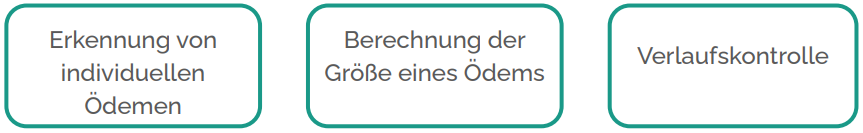
\includegraphics[width=0.7\linewidth]{./pic/Segmentierung/ziel_segmentierung.png}
\caption{\label{fig:ziel_segmentierung}Die drei Ziele, welche im Rahmen der Segmentierung erreicht werden sollen.}
\end{figure}

Diese Ziele können nicht mit der binären Klassifikation erreicht werden. Das folgende Kapitel beschäftigt sich mit dem Verfahren der Instanzsegmentierung, welches für die Erkennung und Ausmessung einzelner Objekte in Bildern entwickelt wurde. 



% ----------------------------
\section{Architektur}
% ----------------------------

CNNs, bereits im Unterabschnitt \ref{CNN} vorgestellt, dienen als Grundlage für die Entwicklung effizienterer Architekturen im Bereich der Bildsegmentierung: insbesondere in der Objekterkennung, Semantischen Segmentierung  sowie Instanzsegmentierung.  

\begin{figure}[H]
\centering
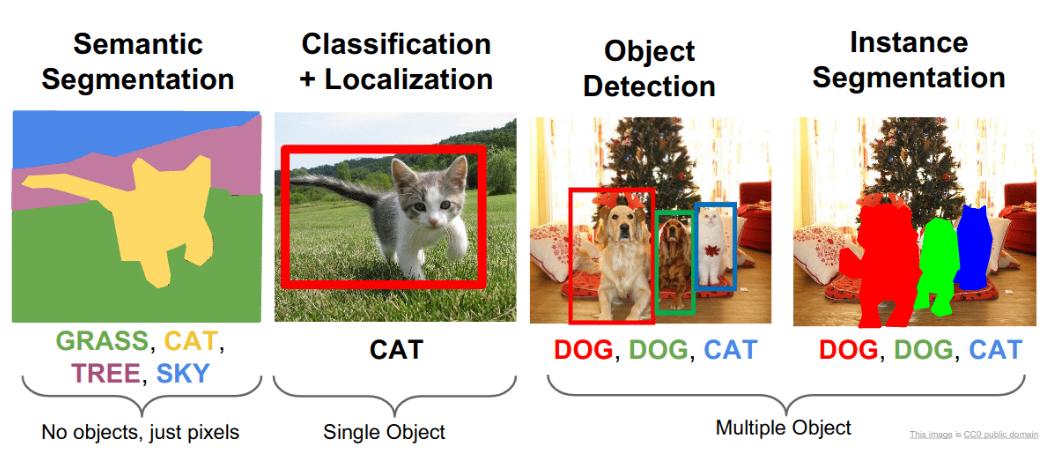
\includegraphics[width=0.7\linewidth]{pic/Segmentierung/segmentation_catsndogs.png}
\caption{\label{pic:catsndogs} Arten der Segmentierung}
\end{figure}


Die erste Architektur der Objekterkennung lässt sich auf Region Based CNN, auch R-CNN genannt, zurückführen. Im Vergleich zu CNNs klassifiziert R-CNN nicht das gesamte Bild, sondern jedes einzelne Objekt in einem Bild. Dabei wird jedes Objekt mit einer Bounding Box versehen und anschließend einzeln in das CNN zur Feature Extraction und Klassifizierung weitergegeben. Die Suche nach sogenannten Region Proposals, also Regionen, wo Objekte enthalten könnten, läuft im R-CNN mit der Selektiven Suche. Da die Suche nach Region Proposals mit der Selektiven Suche sehr zeitaufwendig und ineffizient ist, wurde sie in den folgenden Jahren im Faster R-CNN durch ein Region Proposal Netzwerk (RPN) ersetzt. 

Semantische Segmentierungsverfahren wie z.B. das Fully Convolutional Netzwerk (FCN) sind für das Maskieren der Objekte auf Pixel Ebene verantwortlich. Eine Einschränkung in der Semantischen Segmentierung besteht darin, dass Objekte derselben Klasse in einem Bild nicht voneinander unterschieden werden. Existieren z.B. zwei Katzen in einem Bild, werden alle entsprechende Pixel dem Label Katze zu geordnet und nicht differenziert zwischen Katze 1 und Katze 2.

Die Instanzsegmentierung behebt die Einschränkung der Semantischen Segmentierung. Zudem wird jedes Objekt mit einer Bounding Box lokalisiert. Die Instanzsegmentierung vereint also die Elemente der Objekterkennung mit denen der Semantischen Segmentierung und bietet eine höhere Genauigkeit im Bereich der Bildsegmentierung. 

% ----------------------------
\subsection{Mask R-CNN}
% ----------------------------

Für das Projekt wurde das Mask R-CNN als Architektur der Instanzsegmentierung gewählt, welches Faster R-CNN aus der Objekterkennung mit dem Fully Convolutional Netwerk (FCN) aus der Semantischen Segmentierung in seiner Architektur vereint. Genauer gesagt erweitert das Mask R-CNN die Architektur der Faster R-CNN um den sogenannten mask branch (s. Abb. \ref{pic:mask_rcnn}), um das Maskieren der Objekte zu ermöglichen. 

\begin{figure}[H]
\makebox[\linewidth]{%
  \begin{tabular}{cc}
    Faster R-CNN Architektur & Mask R-CNN Architektur\\
    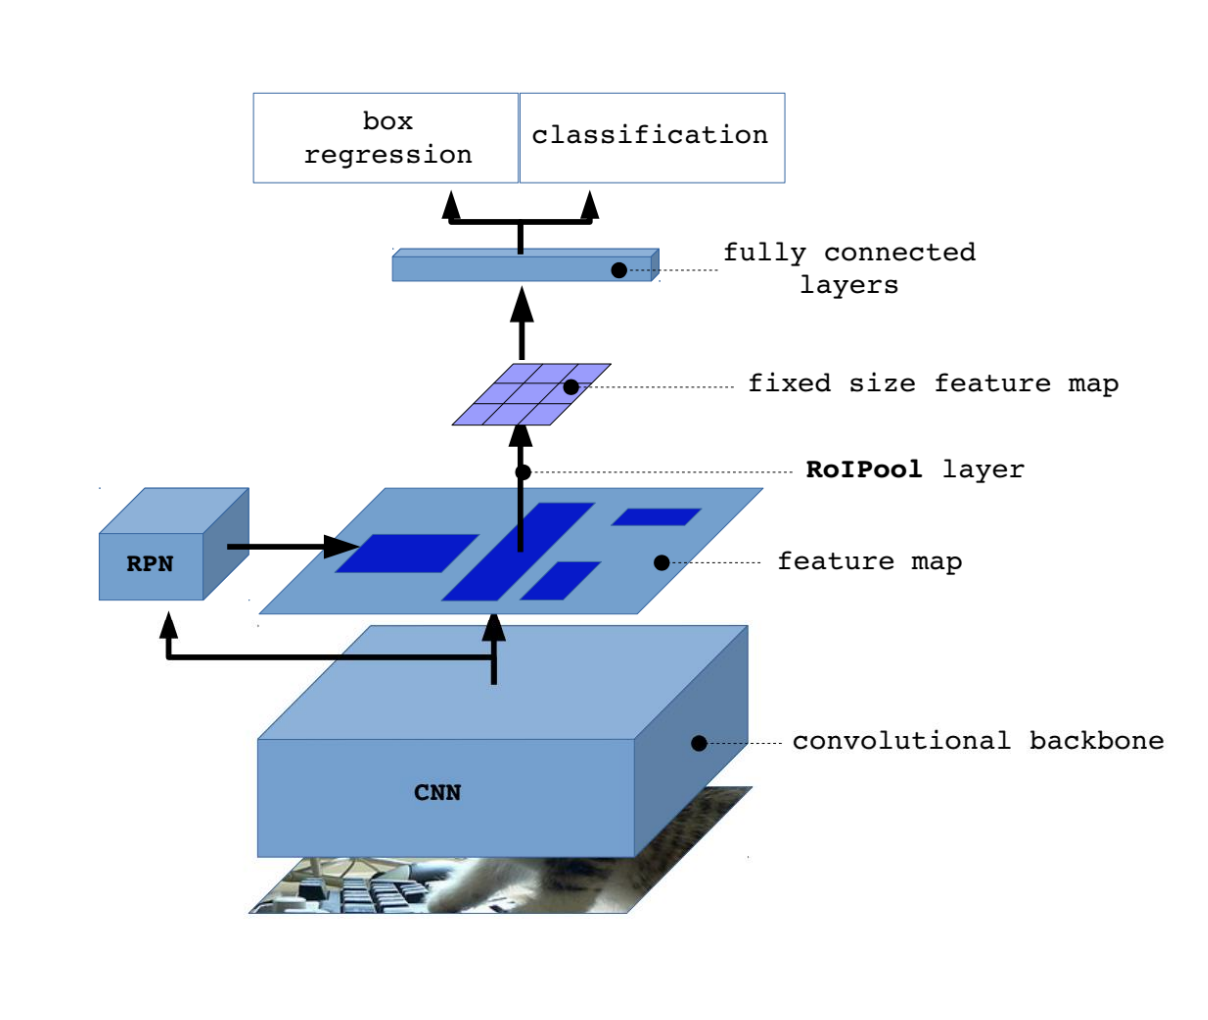
\includegraphics[width=0.4\linewidth]{pic/Segmentierung/faster_rcnn.png}&
    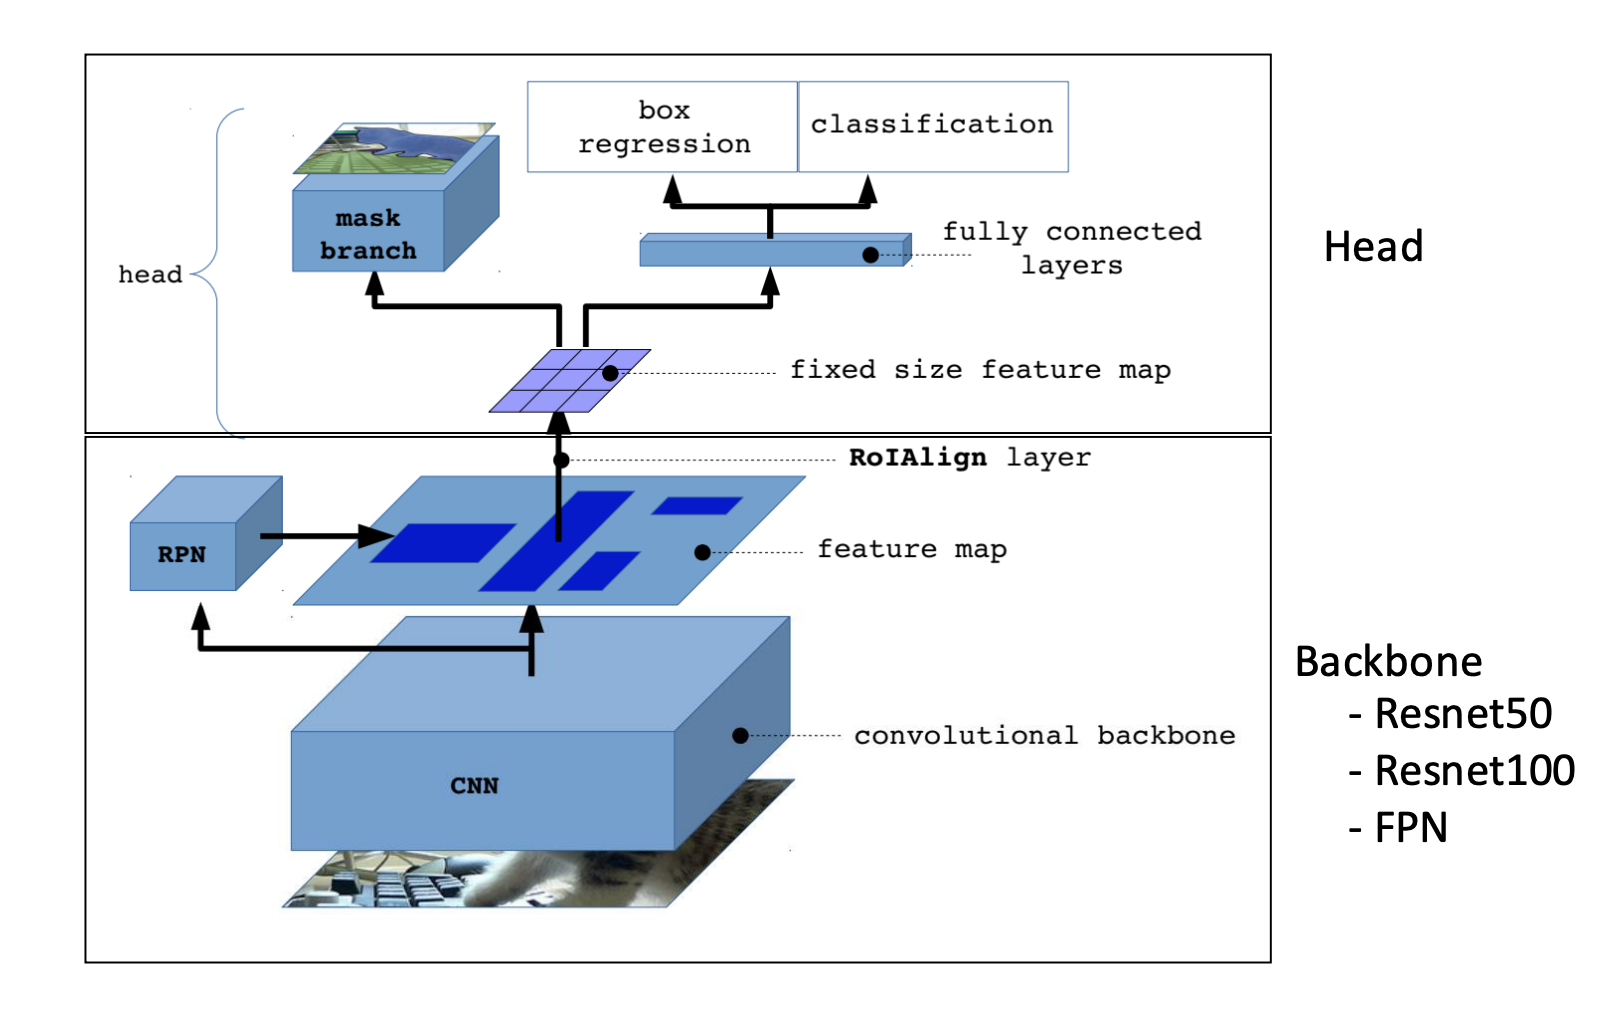
\includegraphics[width=0.5\linewidth]{pic/Segmentierung/mask_rcnn.png}\\
  \end{tabular}%
}
 \caption{Mask R-CNN als Erweiterung des Faster R-CNNs um den Mask Branch}
  \label{pic:mask_rcnn}
\end{figure}

Mask R-CNN ist, wie in \cite{7} und \cite{8} erklärt, ein zweistufiges Verfahren. Die erste Stufe nennt sich Backbone und die zweite heißt Head. Das Backbone enthält ein CNN und ein RPN, mit denen eine Feature Map mit Region Proposals erzeugt wird. Als Backbone Architektur verwendet Mask R-CNN oft ein Resnet50, Resnet100 oder Future Pyramid Netzwerk(FPN). Der Head ist für die Klassifikation und das Maskieren der Objekte verantwortlich.

Um das Konzept des Mask R-CNNs zu verstehen, wird das Vorwissen über CNNs vorausgesetzt, daneben ist das Wissen über das Region Proposal Netzwerk und Fully Convolutional Network von Bedeutung, da sie die wesentlichen Konzepte im Mask R-CNN sind. In den nächsten Unterabschnitten wird auf das Region Proposal Netzwerk (RPN) zur Suche nach Region Proposals (in \ref{subsec:RPN}) und Fully Convolutional Netzwerk (FCN) zum Maskieren der Objekte auf Pixel Ebene (in \ref{subsec:FCN}), eingegangen. Dabei wurde der Unterabschnitt RPN mithilfe von den Quellen \cite{9}, \cite{10} und \cite{11}) verfasst und der Unterabschnitt FCN in Anlehnung an den Arbeiten \cite{12}, \cite{13}, \cite{17}, \cite{18}, \cite{19}, \cite{20} und \cite{21}) erstellt.


% ----------------------------
\subsection{Region Proposal Netzwerk (RPN)} \label{subsec:RPN}
% ----------------------------
Die deutliche Verbesserung in der Laufzeit des Mask R-CNNs im Vergleich zum R-CNN lässt sich vor allem auf das Ersetzen der Selektiven Suche durch das zum Algorithmus integriertes RPN zurückführen. 

Wie ein CNN die Klassifizierung aus der Feature Map lernt, lernt auch RPN Region Proposals aus der Feature Map, dies erfolgt im Wesentlichen in 3 Schritten:

\begin{enumerate}
\item Generiere Anker-Punkte.
\item Generiere Anker-Boxen.
\item Klassifiziere Anker-Boxen in die Klassen Vordergrund (positiv) oder Hintergrund (negativ) und lerne die Abweichungen zwischen der positiven Anker-Boxen und der  Grundwahrheitsboxen.
\end{enumerate}

\begin{figure}[H]
\centering
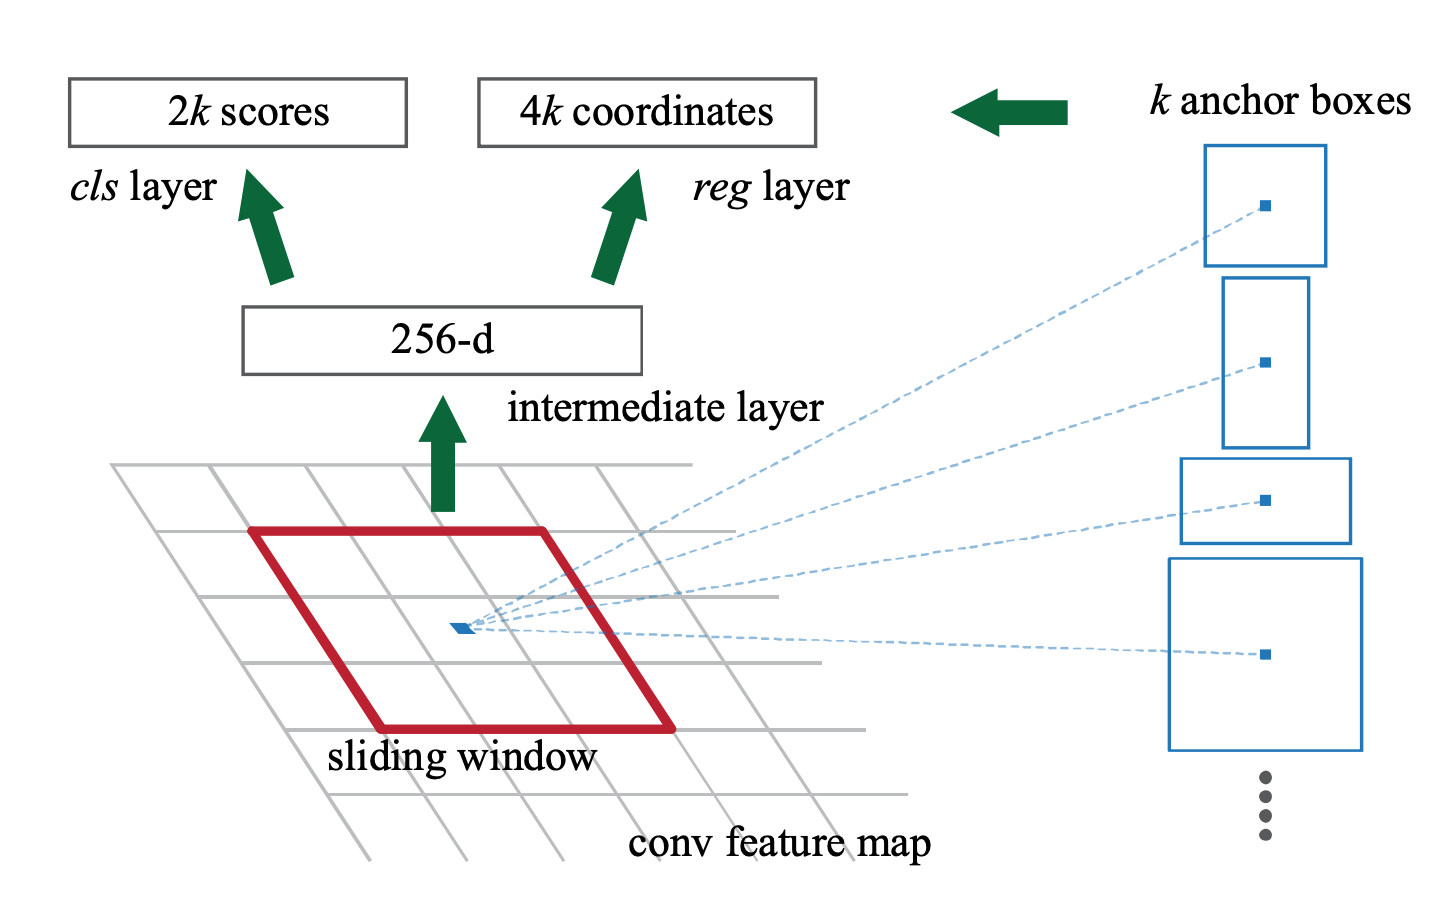
\includegraphics[width=0.5\linewidth]{pic/Segmentierung/RPN_architektur.png}
\caption{\label{pic:rpn} RPN Architektur}
\end{figure}

Die Anker-Punkte werden mit einem gleitenden Fenster (Sliding Window), wie in der obigen Abbildung \ref{pic:rpn} gezeigt, generiert. Die Anzahl der zu generierenden Anker-Punkte hängt von dem Stride des gleitenden Fensters ab, wobei der Stride von der Backbone Architektur entschieden wird. 
\begin{figure}[H]
\centering
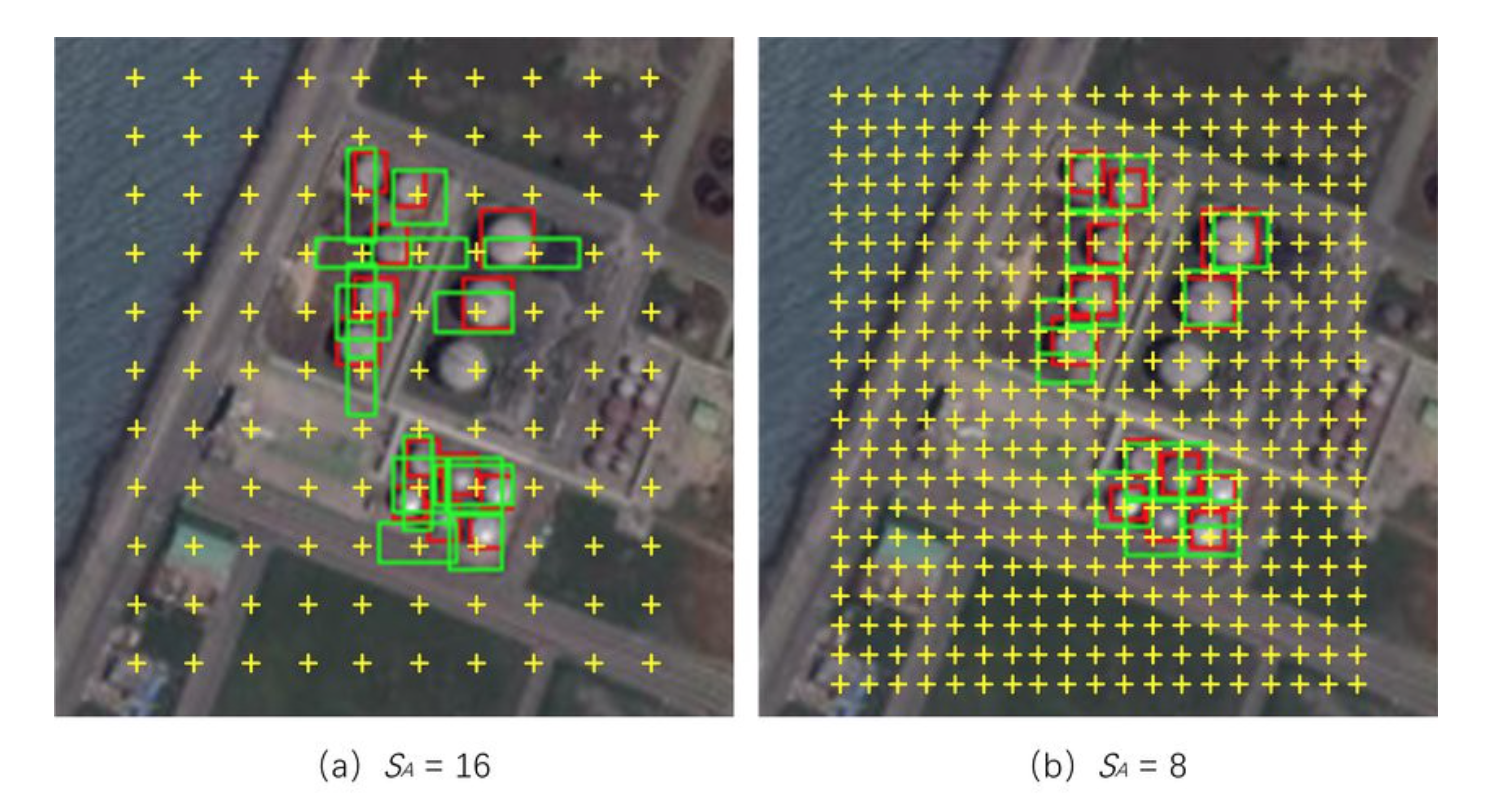
\includegraphics[width=0.7\linewidth]{pic/Segmentierung/Segmentierungsergebnisse/Anker-Punkte.png}
\caption{\label{pic:Anker-Punkte} Anzahl der generierten Anker-Punkte abhängig von dem Stride }
\end{figure}

Nun werden Anker-Boxen verschiedener Größen und Seitenverhältnisse definiert und auf jeden Anker-Punkt gelegt. Im dem ursprünglichen Paper \cite{9} definieren Shaoqing Ren et al. 3 verschiedene Größen: 128$\times$128, 256$\times$256, 512$\times$512 und 3 verschiedene Seitenverhältnisse: 1:1, 1:2, 2:1. Es gibt Anker-Boxen, die Objekte enthalten und Anker-Boxen, die keine Objekte umfassen. Ziel des nächsten Schrittes ist es, Anker-Boxen entsprechend in den Klassen Vordergrund (positiven) und Hintergrund (negativen) zu klassifizieren, dies erfolgt in der Classification Layer (cls layer, s. Abb.\ref{pic:rpn}) und gleichzeitig die Abweichungen zwischen der positiv klassifizierten Anker-Boxen und der Grundwahrheitsboxen in der Regression Layer (reg layer, s. Abb.\ref{pic:rpn}) zu berechnen.

Für die Klassifizierung der Anker-Boxen wird die Intersection over Union (IoU) als Entscheidungsgröße verwendet. 
\begin{Definition}[IoU]
IoU ist eine relative Maßzahl, welche die Stärke der Überschneidung zwischen einer Anker-Box und einer Grundwahrheitsbox beschreibt. Sie ist wie folgt definiert:
\begin{equation}
IoU = \frac{\textrm{Area of Overlap}}{\textrm{Area of Union}}. \label{IoU}  
\end{equation}
\end{Definition}
Die Entscheidungsregel für eine positive Anker-Box auf Grundlage der $IoU$ lautet: Eine Anker-Box mit der höchsten IoU oder mit einer IoU > 0.7 wird positiv klassiziert. Demzufolge erhält jede Anker-Box mit einer IoU < 0.3 ein negatives Label.

Gleichzeitig werden die Koordinaten $x$, $y$, $w$ und $h$ der positiven Anker-Boxen und Grundwahrheitsboxen ermittelt und anschließend deren Differenzen der Koordinaten berechnet. Dabei geben $(x,y)$ die Koordinaten des Mittelpunktes einer Box an und $w$ und $h$ entsprechen jeweils die Breite und Höhe der Box. Die Differenzen werden in der Regression Layer gelernt und minimiert. um die Prognosen der Region Proposals mit Bouding Boxen zu optimieren.

% ----------------------------
\subsection{Fully Convolutional Netzwek (FCN)} \label{subsec:FCN}
% ----------------------------
FCN ist ein Konzept der Semantischen Segmentierung und ermöglicht das Maskieren von Objekten auf Pixel Ebene im Mask R-CNN. FCN lässt sich unterteilen in zwei Phasen: Convolution Netzwerk und Deconvolution Netwerk. 

\begin{figure}[H]
\centering
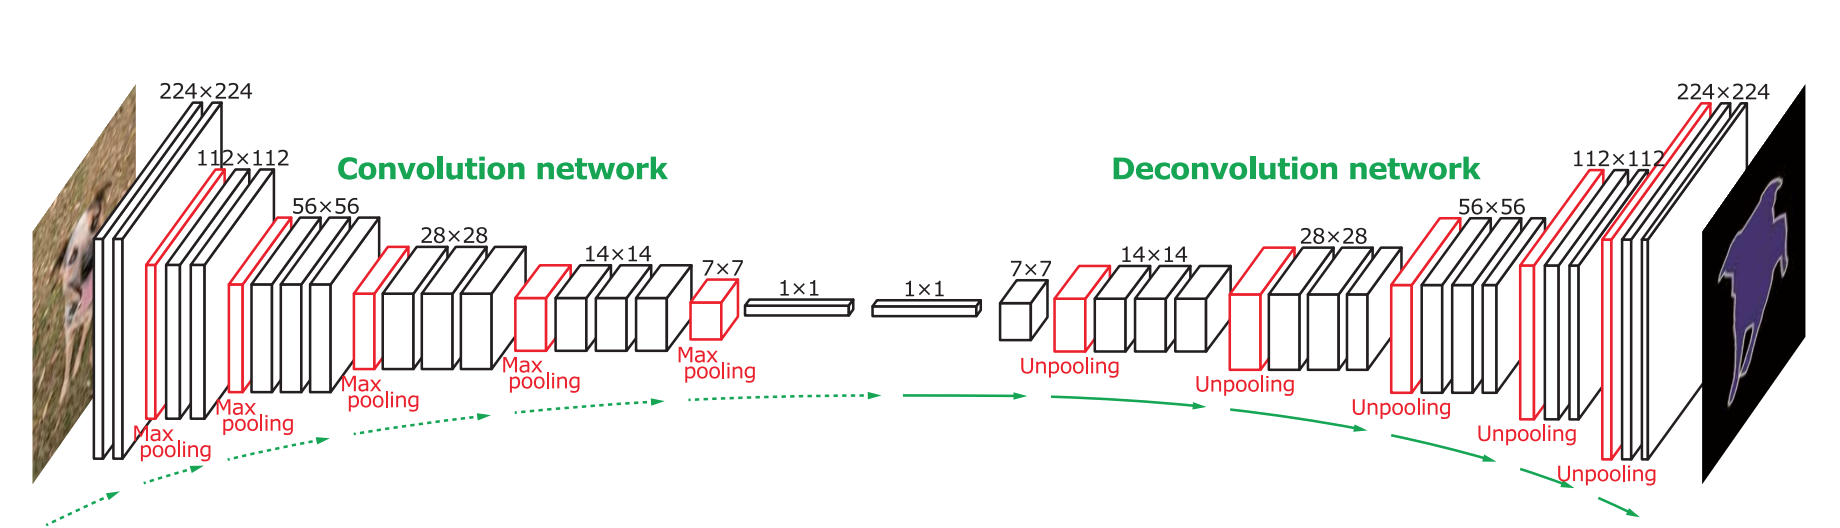
\includegraphics[width=\textwidth]{pic/Segmentierung/ArchitekturFCN.png}
\caption{\label{pic:fcn} Architektur FCN (konkret: VGG-16 Netz)}
\end{figure}

In der ersten Phase wird die räumliche Auflösung des Bildes verkleinert, es wird eine Feature Map erzeugt mit nur wesentlichen Informationen, die das effiziente Lernen von Features zur Klassifizierung auf Pixel Ebene unterstützt. Durch Convolution und Pooling Operationen gehen jedoch die räumlichen Informationen verloren, was das Übertragen der klassifizierten Pixel auf das ursprüngliche Bild Schwierigkeiten bereiten könnte. Diese Schwierigkeit wird in der zweiten Phase im Deconvolution Network mit Unpooling und Transposed Convolution Operationen behoben.


\subsubsection{Convolution Network}
Das Convolution Network ist ähnlich wie das bereits in \ref{CNN} vorgestelltes CNN, es besitzt ebenfalls Convolution Layers, als auch Pooling Layers zum Extrahieren und Lernen von Features. Der einzige Unterschied liegt darin, dass das Convolution Network die Fully Connected Layer im CNN durch eine 1$\times$1 Convolutional Layer ersetzt.  Eine 1$\times$1 Convolutional Layer ist eine 2$d$-Convolution mit einem 1$\times$1$\times$$d$ Kernel, wobei $d$ die Tiefe des Tensor (Input-Matrix) entspricht. Mit dieser Änderung liefert das Convolution Network ein Feature Vektor für jeden Pixel, anstatt ein Feature Vektor für das gesamte Bild wie im CNN. Damit ist die Klassifikation auf Pixel Ebene möglich. Für jedes Objekt wird ein Heatmap geneniert, indem jedes Pixel mit einer Farbintensität gekennzeichnet ist, die die Wahrscheinlichkeit der Anwesenheit des Objektes repräsentiert.


\begin{figure}[H]
\centering
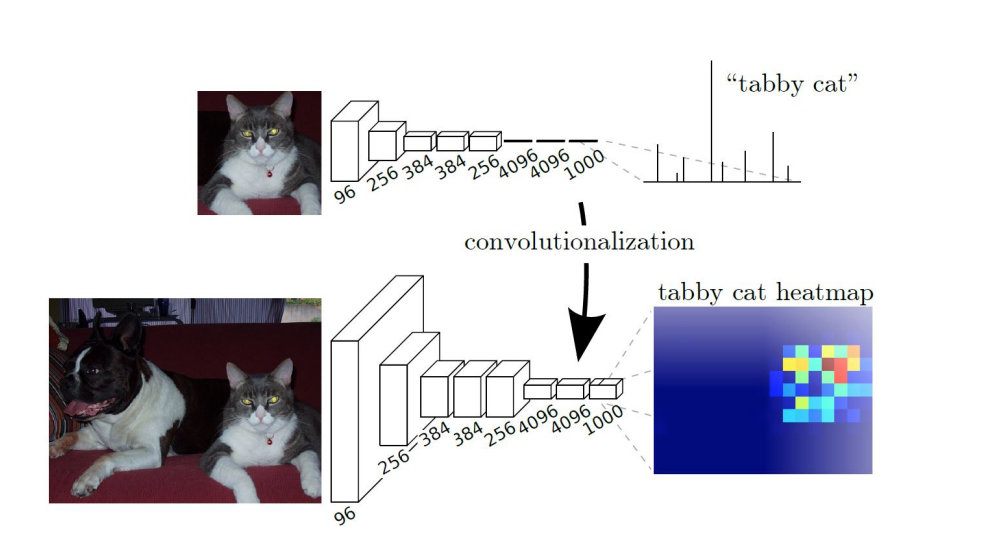
\includegraphics[width=0.8\linewidth]{pic/Segmentierung/Klassifikation_Pixelebene.png}
\caption{\label{pic:class_per_pixel} Klassifikation auf Bildebene vs. Pixelebene}
\end{figure}

\subsubsection{Deconvolution Network}
In dieser Phase geht es darum die geringe Auflösung auf die ursprüngliche Auflösung hochzuskalieren. Dies erfolgt mit den Umkehroperationen (Unpooling und Transposed Convolution) zu denen des Convolution Networks (Pooling, Convolution).

Es gibt verschiedene Unpooling Möglichkeiten: z.B. Nearest Neighbor, Bed of Nails oder Max Unpooling. Beim Nearest Neighbor wird jeder Wert der Input Matrix in die Output Matrix übernommen und gleich oft in die benachbarten Zellen eingefügt.  Beim Bed of Nails wird jeder Wert der Input Matrix in bestimmten Positionen der Output Matrix übernommen und die restlichen Zellen mit Nullen aufgefüllt.
\begin{figure}[H]
\centering
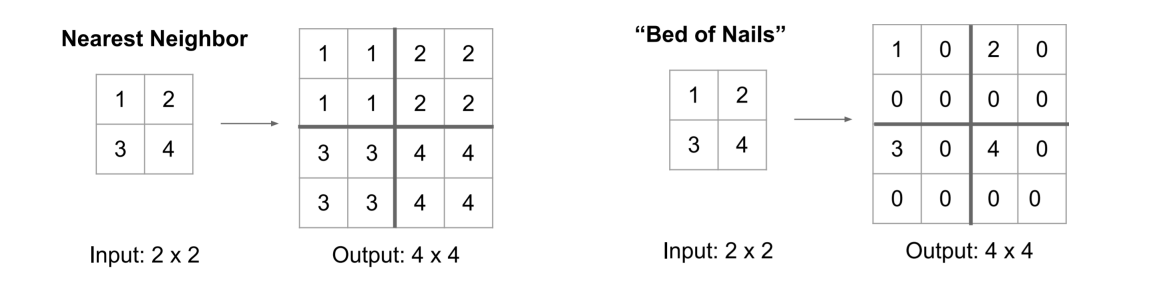
\includegraphics[width=\textwidth]{pic/Segmentierung/NearestNeighbor_BedoofNails.png}
\caption{\label{pic:NN_BoN} Nearest Neighbor und Bed of Nails Unpooling}
\end{figure}
Die Max Unpooling Methode ist die verbesserte Version des Bed of Nails, da die Positionen der Werte in der Output Matrix die Positionen der dazugehörigen Max Pooling Schicht entsprechen. Dies ist möglich wegen der Symmetrie im FCN. 
\begin{figure}[H]
\centering
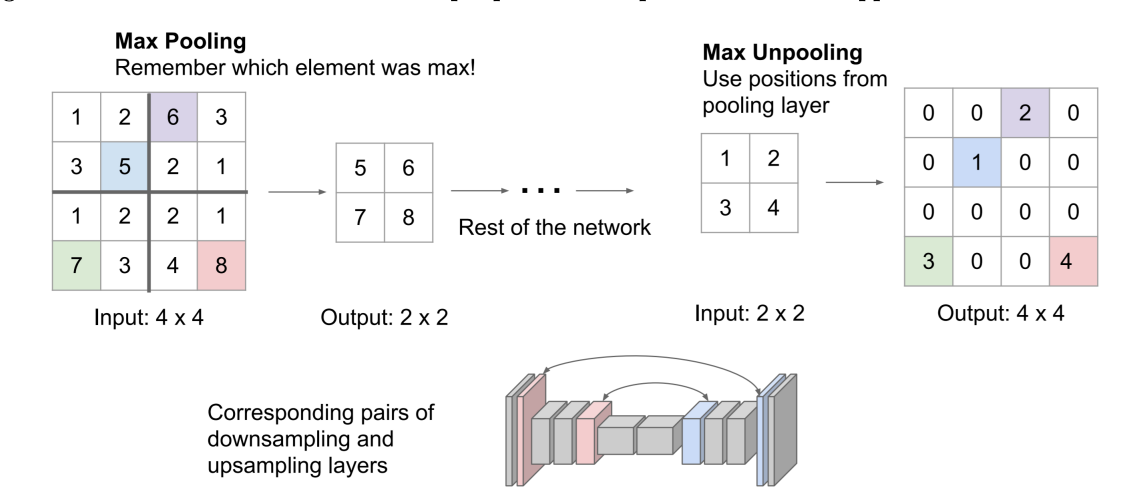
\includegraphics[width=\textwidth]{pic/Segmentierung/MaxUnpooling.png}
\caption{\label{pic:MaxUnpooling} Max Unpooling aufgrund der Symmetrie im FCN}
\end{figure}
Nach dem Unpooling ist die Größe des urspünglichen Tensors wiederhergestellt, wir sehen aber, dass beispielsweise nach dem Max Unpooling noch viele Pixel noch Nullen aufgefüllt sind. Der Informationsverlust wird im Wesentlichen durch Transposed Convolution Operationen behoben. Dabei Zwischentensoren berechnet als Produkt aus der Kernel Matrix und jedes Wertes aus der Input Matrix. Die Zwischentensoren werden anschließend aufsummiert und ergeben die Output Matrix. Die folgende Abbildung illustriert die beschriebene Rechenoperationen.

\begin{figure}[H]
\centering
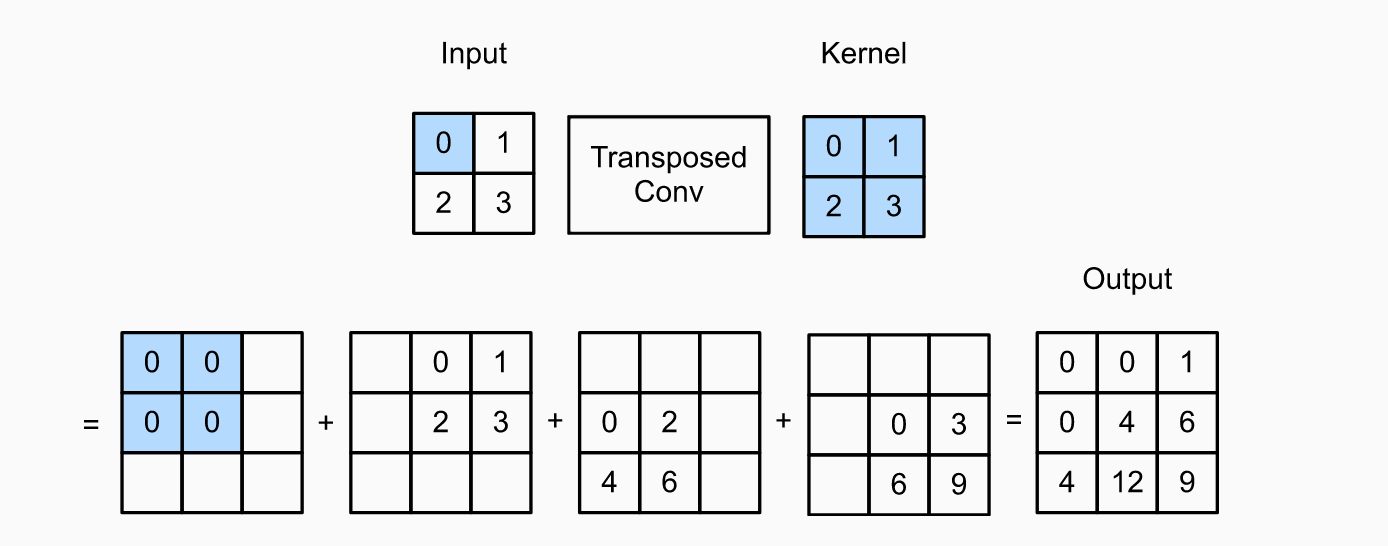
\includegraphics[width=\textwidth]{pic/Segmentierung/TransposedConvolution.png}
\caption{\label{pic:TransposedConvolution} Transposed Convolution mit einem 2x2 Kernel}
\end{figure}

\newpage
\section{Umsetzung}
\subsection{Von den segmentierten Bildern zum trainierten Modell}



Um das Mask R-CNN nicht von Grund auf anlernen zu müssen, wurde ein vortrainiertes Modell als Backbone verwendet. Hierfür wurde das Faster R-CNN ResNet-50 ausgewählt, dass auf dem Common Objects in Context (COCO) Datensatz bereits vortrainiert wurde. 
Der COCO-Datensatz enthält 328 Tausend Bilder mit 80 Objektklassen und 2.5 Millionen gelabelter Segmente. \cite{16}


Der Vorteil der Einbindung des vortrainierten ResNet-50 besteht zum einen darin, dass das ResNet-50 bereits optimiert wurde und somit eine bessere Performance aufweist als ein Modell das von Grund auf erst trainiert werden muss. % hier Beweis/Quelle einfügen
Zum anderen darin, dass mit einer geringen Menge von Bildern gute Resultate im Training erreicht werden können. Da für das Training des Mask R-CNN nur wenige OCT-Bilder zur Verfügung stehen, wirkt sich diese Eigenschaft positiv auf das Ergebnis aus. Die Einbindung des Modells erfolgt über die PyTorch Library.


Nach erfolgreichem Training, können dem Modell nun die Test-Daten übergeben werden, die zur Evaluierung vorgesehen sind.
Auf die Ergebnisse der Evaluierung wird im folgenden Kapitel eingegangen. 

In der folgenden Abbildung \ref{output_mrcnn} ist dargestellt, wie das Ergebnis der Instanzsegmentierung im Output aussieht. 
Auf dem linken Bild ist das korrekt erkannte und gelabelte Ödem mit einer Bounding Box umrahmt. 
Auf der rechten Seite wird das gefundenen Ödem im Bild farblich segmentiert. 

\begin{figure}[H]
\centering
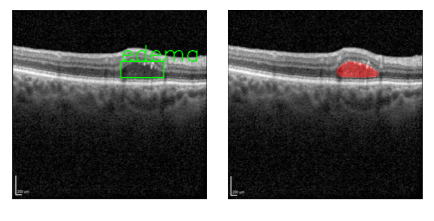
\includegraphics[width=80mm,scale=1.5]{pic/Segmentierung/output_mrcnn.png}
\caption{\label{output_mrcnn}Output Daten des Mask R-CNN (Links: OCT-Bild mit Bounding Box um das gefundene Ödem, Rechts: OCT-Bild mit segmentiertem Ödem)}
\end{figure}



In Abbildung \ref{graph:programmablauf_seg} wird nun aufgezeigt, wie der Programmablauf bei der Erkennung und Segmentierung von Ödemen abläuft.
Dem Segmentierungsmodell wird ein OCT-Bild übergeben. Für das Bild wird durch das Modell eine Vorhersage berechnet, ob Ödeme auf dem Bild vorhanden sind. 
Anschließend werden für alle gefundenen Segmente auf dem Bild die Anzahl der Pixel innerhalb dieser Fläche aufsummiert. 
Abschließend erfolgt dann über das Programm die Ausgabe der Größe des segmentierten Ödems. Die Größenangabe erfolgt hierbei in der Pixelanzahl. 
Wurde kein Ödem auf dem Bild segmentiert, so erfolgt in der Ausgabe eine Größenangabe von 0. 

\begin{figure}[H]
\centering
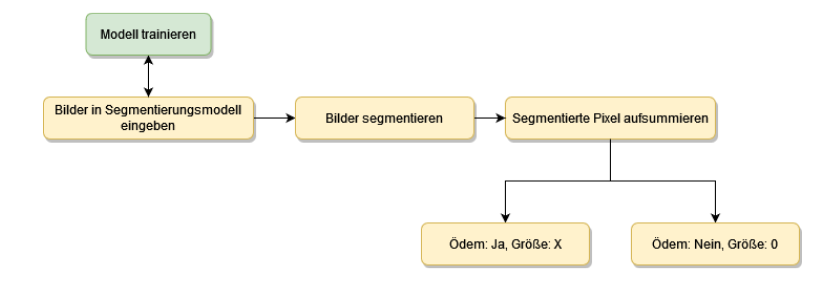
\includegraphics[width=120mm,scale=1.5]{pic/Segmentierung/programmablauf_segmentation.png}
\caption{\label{graph:programmablauf_seg}Programmablauf des Segmentierungsmodells. - \textit{erstellt mit}: \cite{23}}
\end{figure}

\subsection{Erstellen augmentierter Bilder}
Eine Möglichkeit zur Verbesserung der Performanz eines trainierten Modelles ist die Erweiterung des Trainingsdatensatzes \cite{14}. 
Jedoch sind in unserem Anwendungsfall die zur Verfügung stehenden Daten limitiert und es können nicht ohne Weiteres neue Daten erhoben werden.\newline
Um den Trainingsdatensatz ohne die Vermessung weiterer Augen zu erweitern, können Aufnahmen augmentiert werden. Bei der Augmentierung werden die Originalbilder transformiert. Dieselben Transformationen werden dabei an den zugehörigen Masken vorgenommen.\newline
Aufgrund zeitlicher Begrenzung wurde im Rahmen dieses Projektes funktionierender Code zur Datenaugmentierung erstellt, jedoch nicht für das Training verwendet. Als Grundlage für Folgeprojekte wird das Vorgehen in diesem Abschnitt dokumentiert.\newline
Es gibt eine Reihe von Augmentierungsmöglichkeiten. Bei der Auswahl ist es relevant, dass diese auf den konkreten Anwendungsfall passend sind. Daher wurden die Augmentierungsoptionen nach visueller Inspektion aller Patientendaten gewählt.
Insgesamt wurden die folgenden Bildveränderungsmethoden implementiert, welche an einer OCT-Aufnahme in Abb. \ref{fig:segm_augmentiert} visualisiert sind:
\begin{itemize}
    \item Spiegelung an der vertikalen Achse
    \item Drehung um  $\pm$ 15 Grad
    \item Hinzufügen von Rauschen
\end{itemize}

Eine Spiegelung an der vertikalen Achse erweitert den Datensatz auf einfache Weise und ist anatomisch ebenfalls gerechtfertigt, da die Anordnung der Augenschichten durch diese Art der Spiegelung erhalten bleibt. Anders verhält es sich mit der Spiegelung an der horizontalen Achse: Dies ist nicht sinnvoll, da sich ein Makulaödem allgemein über der RPE-Schicht befindet. Bei einer Spiegelung an der horizontalen Achse würde diese lokale Referenz verdreht und die Gefahr eines fehlerhaften Antrainierens der Lage von Ödemen in Relation zu der RPE steigt. Aus dem gleichen Grund sollte eine Drehung der Bilder über 90 Grad vermieden werden. Da die RPE nicht perfekt horizontal sondern in manchen Fällen verkrümmt wirkt, wurde eine Drehung von  $\pm$15 Grad festgelegt. Eine Mögliche Erweiterung wäre eine zufällige Auswahl eines Drehungswinkels im Bereich von $\pm$ 15 Grad um systematische Effekte zu unterdrücken. Da die Augenschichten bei Patienten ungleich sind und eher selten perfekt horizontal im Bild liegen, ist von einem guten Ergebnis auch bei festem Drehwinkel auszugehen. Darüber hinaus besteht durch eine Drehung der Bilder die Möglichkeit, dass antrainierte vertikale Kanten von Segmenten verschwinden und eine dem original nähere Randerkennung erreicht wird. Aufgrund verschiedener Einflussfaktoren wie Alter des Patienten oder weitere Augenerkrankungen werden OCT Bilder verrauschter als bei anderen Patienten. Um die Performanz bei solchen Bildern zu verbessern, wird Gausssches Rauschen auf die Originalbilder, nicht aber auf die Masken hinzugefügt. Die normalverteilten Rauschwerte mit Mittelwert 0 und Standardabweichung 30 werden auf die Pixelwerte addiert. Die resultierenden Pixelwerte werden dabei auf den zugelassenen Bereich von 0 bis 255 begrenzt.
\begin{figure}[h]
\centering
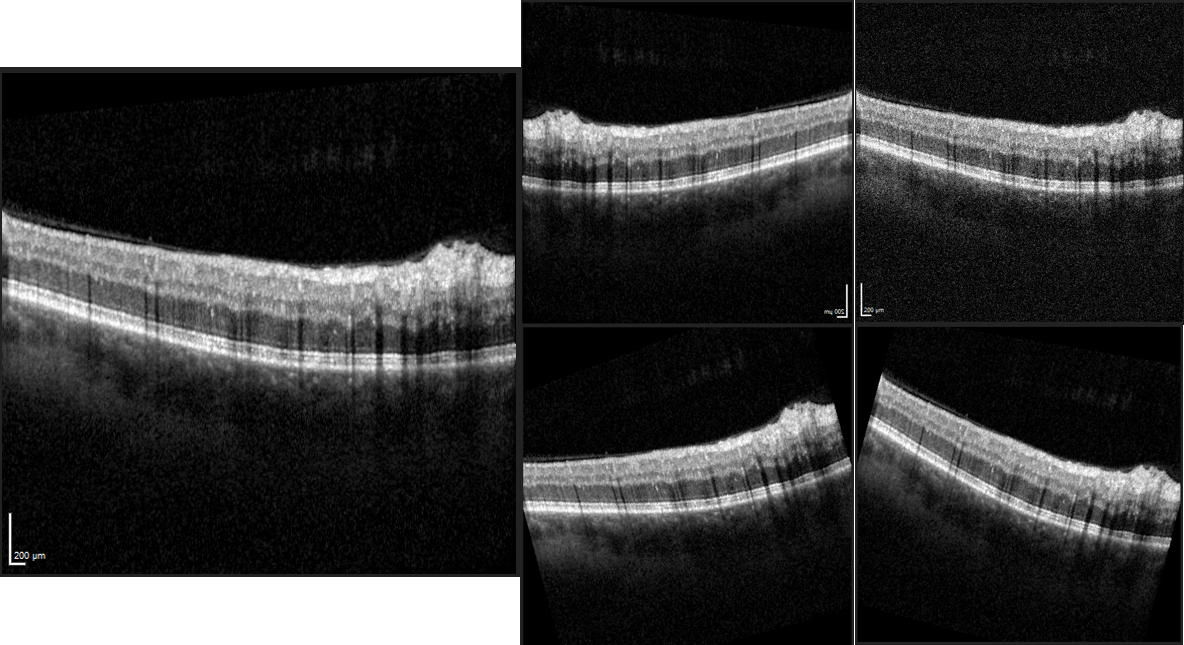
\includegraphics[width=0.5\textwidth]{./pic/Segmentierung/segm_augmentiert.png}
\caption{\label{fig:segm_augmentiert} Bildaugmentierung im Rahmen des Segmentierungstrainings. Links ist das Originalbild zu sehen. Im rechten Viererblock ist links oben die Spiegelung an der Vertikalachse, rechts oben original mit hinzugefügtem Rauschen, links unten Drehung um +15 Grad, rechts unten Drehung um -15 Grad dargestellt.}
\end{figure}


\newpage
\section{Evaluation}
In diesem Kapitel wird das Ergebnis des Segmentierungsmodells anhand der Trainings- und insbesondere Testdaten evaluiert.\newline
Dabei werden sowohl die Kenngrößen bei der Betrachtung des Segmentierungsmodells als binärer Klassifizierer als auch eine feinere Auswertung der Trainings- und Testdaten anhand der Maßzahl IoU vorgestellt.
%%% Strukturnotizen %%%
% IoU
% sensitivity & specificity
% 
\subsection{Segmentierung als binärer Klassifizierer} \label{Segmentierung als binärer Klassifizierer}
%TODO add certainty segmentation
Zu den Ausgabeinformationen der Segmentierung zählen umrandende Boxen ("Bounding Box") sowie Masken gefundener Bereiche. Mithilfe dieser Information kann eine binäre Klassifikation erreicht werden: Wenn mindestens ein Ödem im Bild ermittelt wird und somit mindestens eine Box sicher\footnote{sicher bestimmt gilt ein Ödem, wenn der Parameter \textit{certainty} der zugehörigen Box mindestens 70\% beträgt. Dieser Parameter wurde mithilfe einer Auswertung von Stichproben von uns als passend identifiziert.} bestimmt ist, wird das Bild als "positiv"$\;$klassifiziert. Wenn keine Box sicher ermittelt wurde, wird das Bild als "negativ"$\;$klassifiziert und somit angenommen, dass kein Ödem in dem Bild vorhanden ist.\newline
Insgesamt kann die Evaluation der Klassifizierung auf zwei Ebenen stattfinden: Einerseits auf Bilderebene, bei dem die Klassifikation pro Bild ausgewertet wird. Dabei wird die Auswertung unabhängig von der Zugehörigkeit eines Bildes zum Auge vorgenommen.
Eine weitere Möglichkeit der Evaluation ist die Bewertung auf Augenebene. Dabei wird das Auge eines Patienten, also das Kollektiv aus 25 Bildern, betrachtet. Sobald in mindestens einem Bild der Bilderserie ein Ödem segmentiert wurde, gilt das gesamte Auge als "positiv". \newline
Für diese Evaluation wurden auf Bildebene ausschließlich Testdaten herangezogen, welche nicht im Training gesehen wurden. Somit ergibt sich ein positiver Testdatensatz mit einem Umfang von 50 Bildern, was im Rahmen von Evaluationen eher gering ist. Da dieses Ergebnis somit eine statistische Schätzung mit geringem Stichprobenumfang darstellt, ist dieses Ergebnis in Hinsicht auf die Performanz mit neuen, noch unbekannten Daten im Rahmen des Klinikalltags mit Unsicherheit behaftet.\newline
Wie in Abbildung \ref{fig:barchart_imgeye} erkennbar ist, werden 98\% der Evaluation auf Bildebene korrekt positiv klassifiziert. In absoluten Zahlen wurde somit nur in einem von fünfzig Bildern fälschlicherweise kein Ödem erkannt. \newline
Auf Bilderebene liegt die Falsch-Negativ-Rate bei 9\%, was bei einem Testdatenumfang von 26607 Bildern als aussagekräftig zu bewerten ist.

\begin{figure}[ht!]
\centering
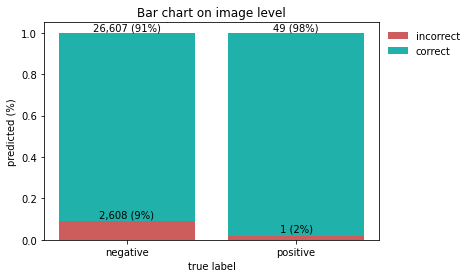
\includegraphics[width=0.49\textwidth]{./pic/Segmentierung/barchart_image.png}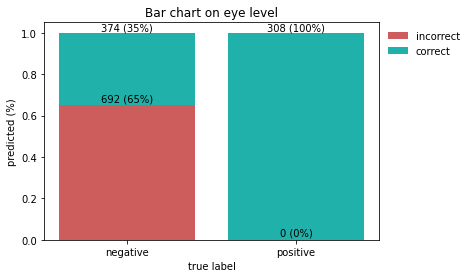
\includegraphics[width=0.49\textwidth]{./pic/Segmentierung/barchart_eye.png}
\caption{\label{fig:barchart_imgeye} Evaluierung der Segmentierung als binärer Klassifizierer auf Bildebene (links) und Augenebene (rechts). Korrekte Klassifikationen sind türkis, inkorrekte rot eingefärbt.}
\end{figure}
Auf Augenebene weichen die Ergebnisse im Vergleich zur Bildebene ab: Alle tatsächlich positiven Augen wurden korrekt als positiv klassifiziert. Dieser Effekt erklärt sich durch die festgelegte Regel, dass bei mindestens einem positiven Bild eines Auges das gesamte Auge als positiv klassifiziert wird, sowie der Tatsache, dass in dieser Evaluation auch Trainingsdaten enthalten sind. 
In dem Szenario der Makulaödemerkennung ist eine Erkennung positiver Fälle wünschenswert: Im Rahmen einer unterstützenden Diagnose ist deutlich schlechter zu bewerten, wenn ein Auge fälschlicherweise als negativ erkannt wird, da somit eine Behandlung des Patienten unter Umständen erst bei einem Folgetermin und somit später als nötig beginnt. Der beste Fall ist es, wenn vorhandene Ödeme stets erkannt werden. Der Anteil von Augen, welcher fälschlicherweise als positiv erkannt wurde, liegt bei etwa 65\%. Eine weitere Untersuchung ergab, dass ein Großteil der falsch positiv klassifizierten Augen aufgrund von zwei oder weniger falsch positiven Bildern fehlklassifiziert wurden.\newline
Diese Ergebnisse führen zu den bereits eingeführten Kennwerten Sensititvität und Spezifität (s. Tab. \ref{tab:sensspec}). Wie auch das Klassifikationsmodell mit Efficient Net wird auch bei der Klassifikation durch das Mask R-CNN eine Sensitivität von 0.98 erreicht. Dabei ist jedoch zu beachten, dass der Wert des Segmentierungsmodells aufgrund des geringen Testdatenumfangs mit Unsicherheit behaftet ist. Darüber hinaus ist die Spezifität des Segmentierungsmodells mit 0.91 sogar besser als jene des Klassifizierers mit 0.82. Aus diesem Grund und aufgrund der Tatsache, dass die Kombination beider Modelle zu tendenziell mehr falsch negativen Fällen führt, wird nur das Segmentierungsmodell in den finalen Prototypen aufgenommen.
\begin{table}[H]
\begin{center}
\begin{tabular}{ l | r | r }
   & Segmentierung Mask R-CNN & Klassifikation Efficient Net \\\hline
 Sensitivität & 0.98 & 0.98 \\  
 Spezifität & 0.91 & 0.82    
\end{tabular}
\caption{\label{tab:sensspec} Sensitivität und Spezifität der Klassifikation auf Bilderebene. Dabei werden die Ergebnisse des Segmentierungsmodells in Funktion eines binären Klassifizierers mit dem Klassifikationsmodell des Efficient Net verglichen.}
\end{center}
\end{table}
% TODO Nachweis
% TODO TO DECIDE schreiben, dass tp eig mist ist?

\subsection{Intersection over Union (IoU)}
Um die Güte eines Segmentierungsresultates zu beschreiben, reichen bisherige Kennzahlen wie Sensitivität und Spezifität nicht aus. Vielmehr muss die Lage und Größe des vom Modell bestimmten Segments mit Lage und Größe des wahren Segments verglichen werden. Eine Kennzahl hierfür ist die Intersection over Union (IoU).
\subsubsection{IoU als Maßzahl}
In diesem Kapitel wird die bereits in Definition \ref{IoU} eingeführte Kenngröße IoU anschaulich gezeigt um die Interpretation der Ergebnisse zu unterstützen.\newline
Im Folgenden wird allgemein von zwei Flächen gesprochen. Auf das Segmentierungsergebnis übertragen repräsentiert eine Fläche die wahre, von Hand segmentierte Fläche und die Andere die Segmentierung des Modells.\newline
Die Intersection over Union wird in Abbildung \ref{fig:iou} visualisiert. Diese setzt den Schnitt beider Flächen, also die gemeinsame Fläche, in das Verhältnis zur Vereinigung. Eine IoU von 1 repräsentiert ein perfektes Ergebnis, bei dem das vom Modell bestimmte Segment exakt dem von Hand markierten Bereich entspricht. Hingegen ist eine IoU von 0 ein Zeichen einer stark fehlerhaften Segmentierung, welche entweder vom Modell an falscher Stelle vorgenommen wurde oder wenn gar kein Segment erkannt worden ist.

\begin{figure}[H]
\centering
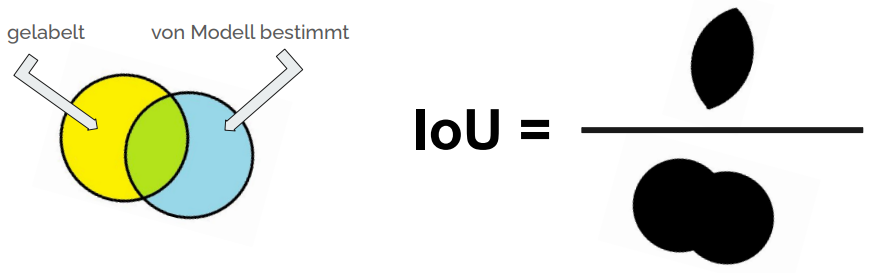
\includegraphics[width=\textwidth]{./pic/Segmentierung/iou.png}
\caption{\label{fig:iou}Zusammensetzung der Kennzahl Intersection over Union (IoU): Dabei wird das Verhältnis von Durchschnitt zu Vereinigung der von Hand segmentierten Fläche und von Modell erkannten Fläche gebildet.}
\end{figure}

Darüber hinaus kann die Aussagekraft der IoU von weiteren Faktoren beeinflusst werden. Eine solcher Einflussfaktor ist die Größe der segmentierten Flächen: Durch das Bilden eines Verhältnisses haben kleine absolute Abweichungen von kleinen Flächen ein höheres Gewicht als bei großen Flächen. Somit ist zu erwarten, dass die IoU bei kleinen Segmenten tendenziell schlechter ausfällt obwohl die subjektive Segmentierungsqualität in etwa gleich wirkt. Somit kann es sinnvoll sein, die Größe bei der Evaluierung der Qualität anhand der IoU zu berücksichtigen. Zudem spielt der Faktor Mensch eine Rolle: Die Segmentierung von Hand wurde von unterschiedlichen Personen durchgeführt. Trotz anfänglicher Absprache kann es auch hier zu unterschiedlichen Arten der händischen Segmentierung kommen. Darüber hinaus wurden die Bilder von Data Science Studierenden und nicht von medizinischem Fachpersonal durchgeführt, weswegen es trotz Hilfestellung von Augenärzten zu Fehlsegmentierungen in den Originalbildern kommen kann.

%TODO remove newpage

\subsubsection{IoU der Trainings- und Testdaten}

Bei einer Auswertung der IoU des Testdatensatzes (Abb. \ref{fig:iou_testonly50}) zeigt sich, dass der Median der IoU bei 0.70 und der Mittelwert bei 0.63 liegt.\newline
Auf einem Testbild wurde kein Segment erkannt, was zu einer IoU von 0 führt.
% TODO mehr ausfuehren
Aufgrund des Umfangs von 50 positiven Testbildern wirkt das Histogramm nicht glatt. Nichtsdestotrotz zeigt sich eine Häufung von Bildern in einem IoU Bereich von 0.4 bis etwa 0.9.

\begin{figure}[H]
\centering
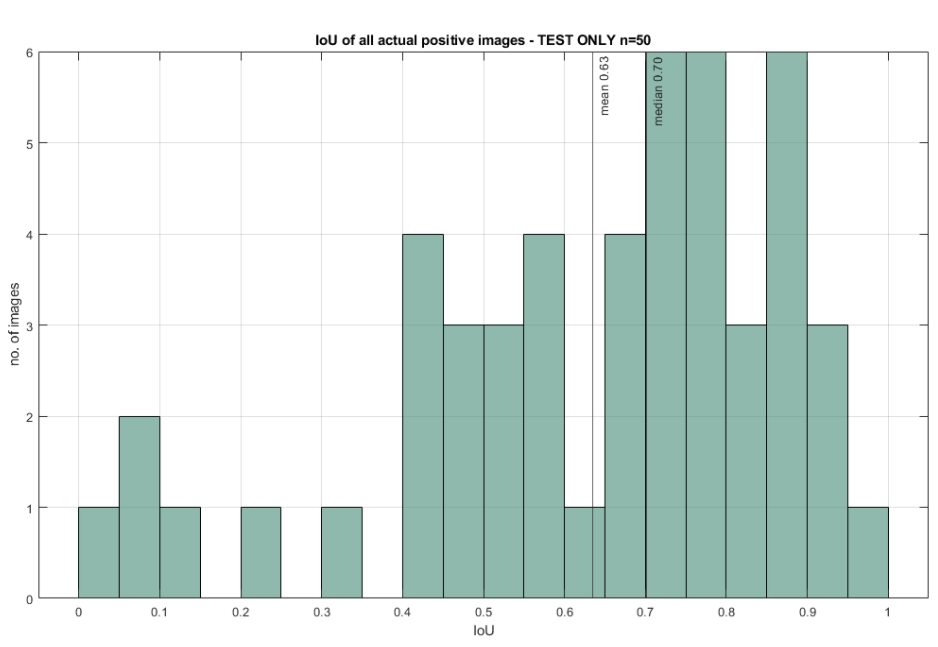
\includegraphics[width=\textwidth]{./pic/Segmentierung/iou_testonly50.png}
\caption{\label{fig:iou_testonly50}Histogramm der Intersection over Union als Ergebnis der Evaluation aller positiven Testdaten. Auf der Abszisse ist die Intersection over Union, auf der Ordinate die Anzahl der Bilder aufgetragen.}
\end{figure}

Im Median liegt bei der Evaluation der positiven Bilder eine IoU von 0.74 vor. Somit wird bei der Hälfte der Ergebnisbilder eine IoU kleiner als 0.74, der anderen Hälfte eine IoU größer als dieser Wert zugeordnet. Wie erwartet, wurde bei keinem Bild eine IoU von 100\% erreicht. \newline

Da der Testdatenumfang mit 50 Bildern gering ist, wurde in einem weiteren Evaluationsschritt neben den Testdaten auch die Trainingsdaten herangezogen. Dabei ist zu beachten, dass diese Ergebnisse eher eine Obergrenze zur Performanz auf neuen, unbekannten Daten darstellen. Das heißt, dass die tatsächliche Performanz des Modelles auf neuen Daten generell schlechter sein wird als die folgenden Bilder zeigen.\newline
Bei der Auswertung von sowohl Trainings- als auch Testdaten (s. Abb. \ref{fig:iou_testonly50})  zeigt sich, dass sowohl Median (0.74) als auch Mittelwert (0.66) etwas höher sind im Vergleich zu der Auswertung der Testdaten. Dieser Effekt ist dadurch erklärbar, dass Trainingsdaten dem Modell bereits bekannt sind und somit tendenziell besser abschneiden. Die Abweichung ist jedoch nicht extrem, was ein Hinweis auf eine gute Performanz des Modells auf unbekannten Daten ist.


\begin{figure}[H]
\centering
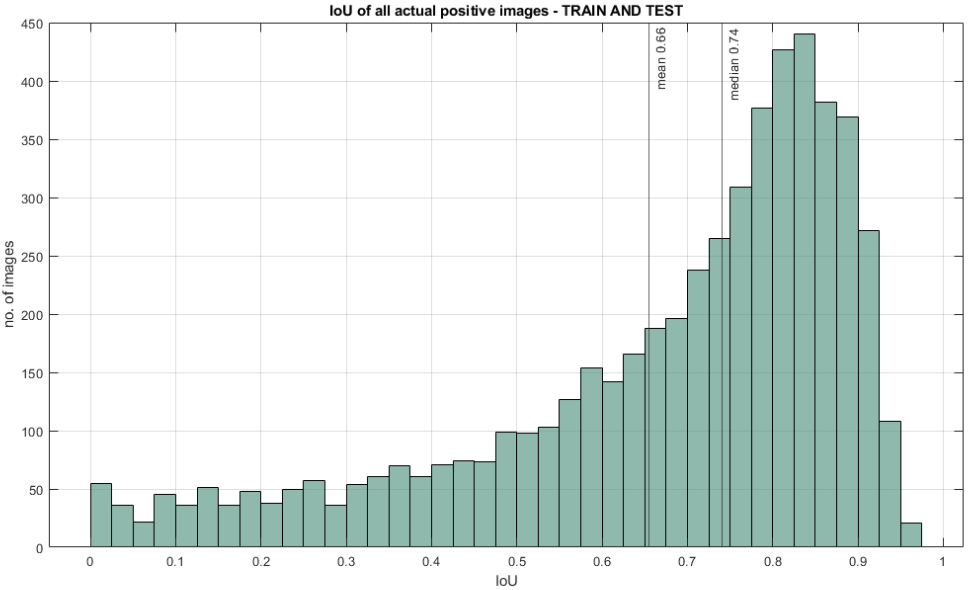
\includegraphics[width=0.8\textwidth]{./pic/Segmentierung/iou_pos_traintest.png}
\caption{\label{fig:iou_pos_traintest}Histogramm der Intersection over Union (IoU) als Ergebnis der Evaluation aller original positiven Bilder. Dabei sind sowohl Trainings- als auch Testbilder berücksichtigt. Auf der Abszisse ist die Intersection over Union, auf der Ordinate die Anzahl der Bilder aufgetragen.}
\end{figure}

Bei einer Betrachtung der Auswertung pro Größenintervall (Abb. \ref{fig:iou_pos_traintest_persize}) werden die zuvor aufgestellten Hypothesen bestätigt: Es zeigt sich, dass die Werte der Lagemaße der IoU bei kleinen Segmenten (weniger und gleich 800 Pixel) geringer sind als bei größeren Ödemen. Darüber hinaus ist die Streuung der im Histogramm dargestellten Verteilungen bei kleinen Segmenten größer als bei mittelgroßen oder großen Segmenten. Das bedeutet nicht zwingend, dass große Ödeme von dem Modell besser segmentiert werden sondern kann auf die Berechnung der IoU zurückgeführt werden.

\begin{figure}[H]
\centering
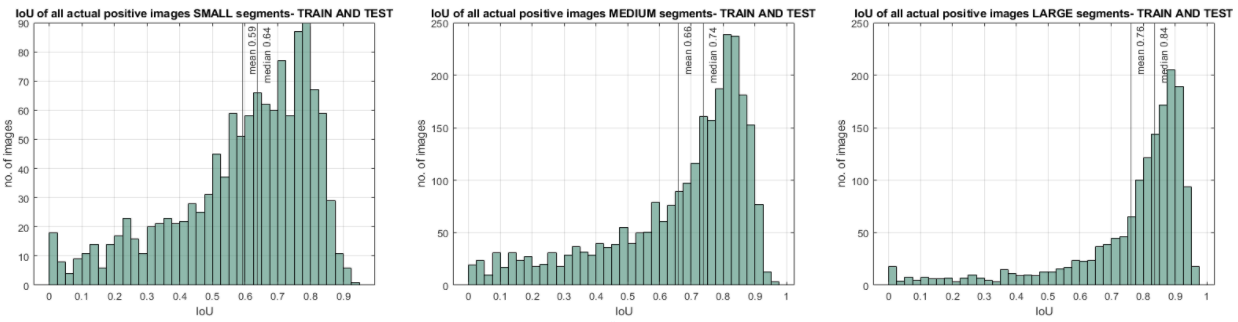
\includegraphics[width=\textwidth]{./pic/Segmentierung/iou_pos_traintest_persize.png}
\caption{\label{fig:iou_pos_traintest_persize}Histogramm der Intersection over Union (IoU) als Ergebnis der Evaluation aller original positiven Bilder. Insgesamt sind drei Histogramme zu sehen, welche sich in der Größe der segmentierten Ödeme unterscheiden. Links ist das Histogramm kleiner Ödeme (kleiner gleich 800 Pixel), in der mittleren Darstellung mittelgroße Ödeme (ab 801 bis 10.000 Pixel), rechts große Ödeme (größer als 10.000 Pixel) dargestellt. Dabei sind sowohl Trainings- als auch Testbilder berücksichtigt. Auf der Abszisse ist die Intersection over Union, auf der Ordinate die Anzahl der Bilder aufgetragen.}
\end{figure}
\newpage
\subsection{Anzahl segmentierter Pixel tatsächlich negativer Bilder}
Da bei tatsächlich negativen Bildern die von Hand segmentierte Fläche nicht vorhanden ist, kann diese Metrik zur feineren Beurteilung der Performance des Modells nicht herangezogen werden. Möglich ist hingegen die Evaluation der Größe fälschlich segmentierter Flächen durch die Anzahl der segmentierten Pixel im Bild.\newline

\begin{figure}[H]
\centering
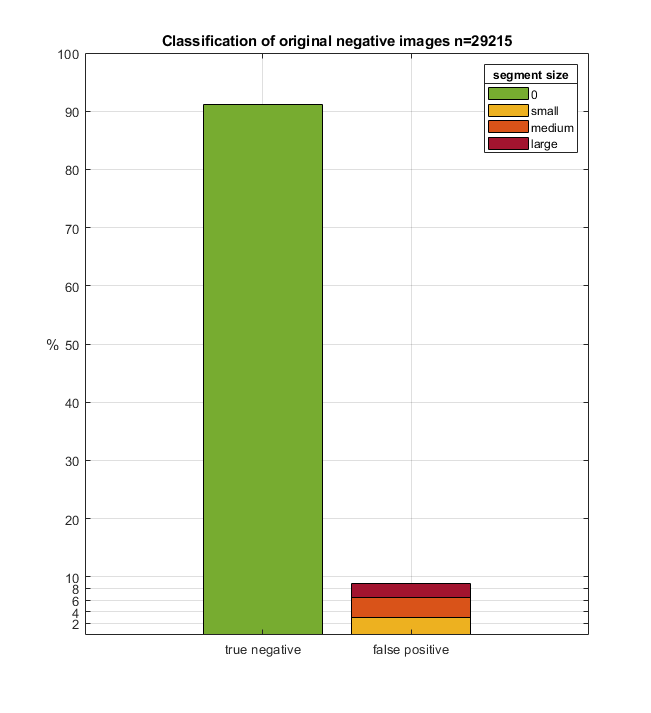
\includegraphics[width=0.7\textwidth]{./pic/Segmentierung/trueNeg_fp_imglevel_n.png}
\caption{\label{fig:trueneg}Darstellung der Anzahl vom Modell segmentierter Pixel tatsächlich negativer Bilder. Links sind die wahren, negativen Bilder dargestellt, rechts alle fälschlich als positiv klassifizierten Bilder. Die Farbcodierung zeigt das Intervall segmentertier Pixel in rot (Größer als 10.000 Pixel), orange (zwischen 800 und 10.000 Pixel) und gelb (weniger als 800 Pixel).}
\end{figure}
In Abb. \ref{fig:trueneg} ist diese Aufteilung visualisiert. Es wird wieder deutlich, dass mit 91\% bei den meisten tatsächlich negativen Bildern vom Modell keine Segmentierung vorgenommen wird. Insgesamt werden in 3\% tatsächlich negativer Bilder kleine Ödeme unter 800 Pixel gefunden, in 4\% der Bilder mittelgroße Ödeme zwischen 800 und 10.000 Pixeln , und in 2\% der Fälle große Ödeme größer als 10.000 Pixel segmentiert.\newline
Diese Information sollte bei der Bewertung der Verlaufskontrolle beachtet werden, da insbesondere große fälschlich erkannte Segmente zu Fehlern in der ermittelten Ödemgröße führen können.


\newpage
\subsection{Auszug von Ergebnisbildern}
Nachdem die Evaluation der Testdaten quantitativ vorgenommen wurde, wird in diesem Kapitel ein Auszug der Testdatenbilder gezeigt. Dabei kann visuell die Größe IoU und die Güte des Segmentierungsergebnisses in Zusammenhang gebracht werden.\newline
Im Folgenden werden die drei Testbilder dargestellt, welche die geringste IoU des Testdatensatzes aufwiesen. In der jeweiligen Teilüberschrift sind die ursprüngliche Bezeichnung des Bildes, die Anzahl vom Modell segmentierter Pixel sowie die berechnete IoU aufgeführt. Rechts wird die Größenklasse angezeigt, in die das vom Modell segmentierte Ödem fällt. Dabei gibt es die Größenklassen 'small', 'medium' und 'large'. Alle drei gezeigten Bilder weisen auf Schwächen des Segmentierungsmodells hin.\newline
In Abb. \ref{fig:ergebnis_notgood1} wurde von dem Modell kein Ödem gefunden. Tatsächlich ist ein Ödem vorhanden. Dieser Fall tritt nur bei einem von den insgesamt 50 Testbildern auf.\newline
\begin{figure}[H]
\centering
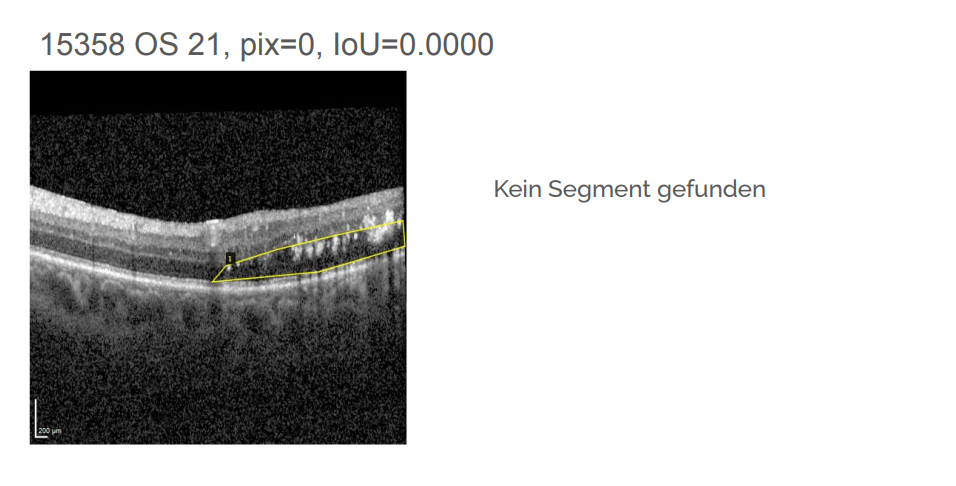
\includegraphics[width=0.75\textwidth]{./pic/Segmentierung/Segmentierungsergebnisse/1.PNG}
\caption{\label{fig:ergebnis_notgood1}Evaluiertes Testbild, bei dem vom Modell Ödem segmentiert wurde. Links von Hand segmentiert, rechts Output des Segmentierungsmodells.}
\end{figure}

Eine weitere Schwäche zeigt sich in Abbildung \ref{fig:ergebnis_notgood2}: Ein kleines Ödem wurde nicht erkannt, dafür aber ein relativ großer Abschnitt einer sichtbaren Hyperreflektivität. Letztere zeichnet sich ähnlich wie ein Ödem durch eine dunklere Abbildung aus, man sieht jedoch, dass die RPE in diesem Bereich ebenfalls dunkler aussieht. Durch gezieltes Training könnte diese Schwäche eliminiert werden. Für die bewertenden Ärzte ist es jedoch von Relevanz zu wissen, dass das Ausmessen solcher Fälle durch das Modell fehlerhaft sein kann.\newline
\begin{figure}[H]
\centering
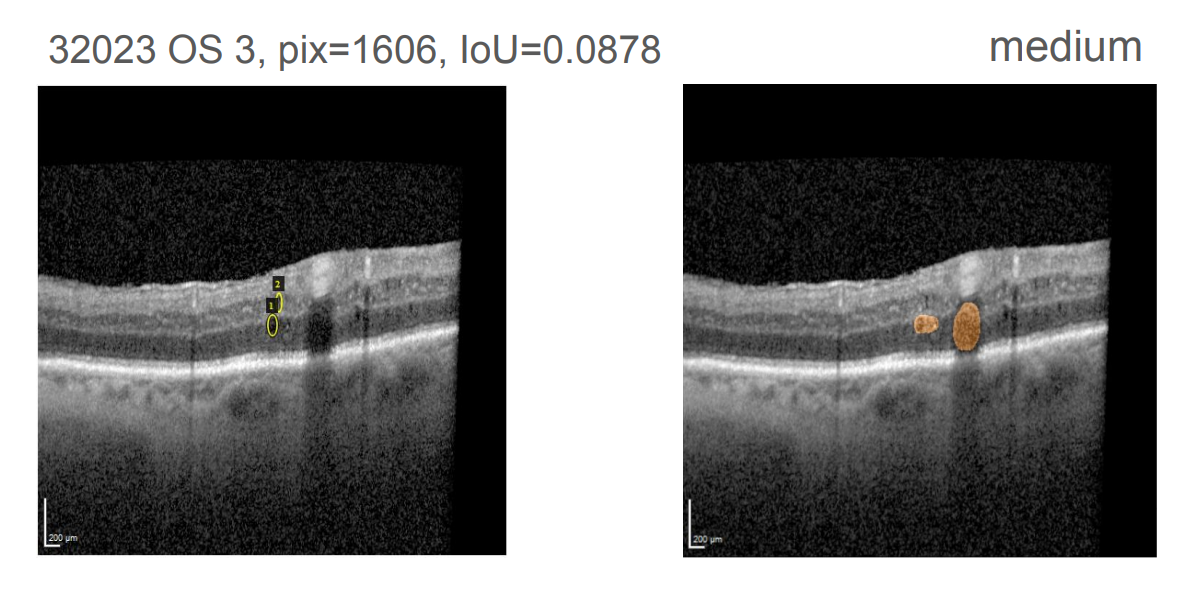
\includegraphics[width=0.75\textwidth]{./pic/Segmentierung/Segmentierungsergebnisse/2.PNG}
\caption{\label{fig:ergebnis_notgood2}Evaluierte Testbild, welches eine geringe IoU und Fehlsegmentierung im Bereich einer Hyperreflektivität aufweist. Links von Hand segmentiert, rechts Output des Segmentierungsmodells.}
\end{figure}

Als dritte Schwäche zeigt sich die fälschliche Markierung eines Ödems unterhalb der RPE, was in Abbildung \ref{fig:ergebnis_notgood3} erkennbar ist. Ein solcher Fehler kann vor Allem in der Ausmessung und somit im Rahmen des Größenverlaufes zu verfälschten Ergebnissen und Missinterpretaitionen führen. Bei weiteren Testbildern mit ähnlicher Abbildung wurden nur Ödeme oberhalb der RPE identifiziert. Dies deutet an, dass der Fehler eher selten vorkommt.\newline
\begin{figure}[H]
\centering
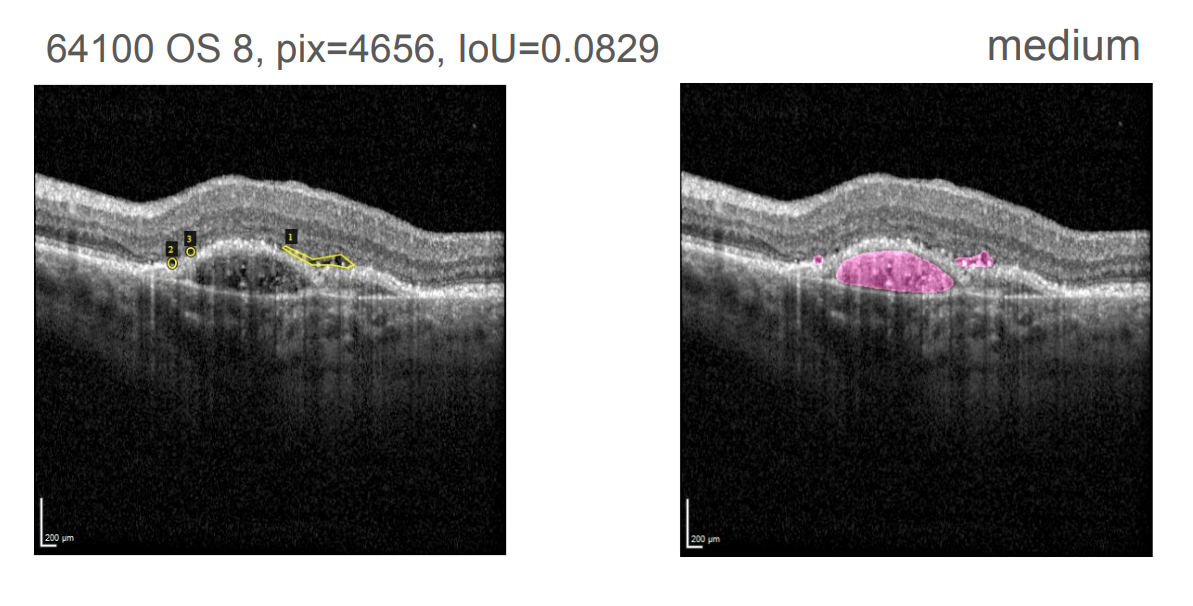
\includegraphics[width=0.75\textwidth]{./pic/Segmentierung/Segmentierungsergebnisse/3.PNG}
\caption{\label{fig:ergebnis_notgood3}Evaluiertes Testbild, welches eine geringe IoU und Fehlsegmentierung aufweist. Links von Hand segmentiert, rechts Output des Segmentierungsmodells.}
\end{figure}

Nachdem eim Auszug der weniger guten Ergebnisse vorgestellt wurde, werden nun Beispiele unterschiedlicher Größen und IoUs gezeigt um einen Eindruck der Resultate der Segmentierung zu gewinnen.\newline
Wieder ist auf der linken Seite jeweils das mithilfe des Image Annotators segmentierte Bild zu sehen, auf der rechten Seite das Ergebnis des Segmentierungsmodells. Dieser Auszug umfasst Bilder mit unterschiedlich großen Segmenten sowie unterschiedlicher IoU.\newline
In Abbildung \ref{fig:ergebnis_good1} ist ein kleines Ödem erkennbar, welches vom Segmentierungsmodell qualitativ gut erkannt wurde. Nichtsdestotrotz ist die IoU mit etwa 0.64 eher im mittleren Bereich einzuordnen. Die geringe IoU kann sowohl aus der geringen Größe resultieren, als auch durch die Verwendung einer Ellipse zur händischen Segmentierung, obwohl das Ödem nicht perfekt elliptisch ist. Fachkräfte stuften dieses Ergebnis im Rahmen der Abschlusspräsentation jedoch als gut ein.
\begin{figure}[h]
\centering
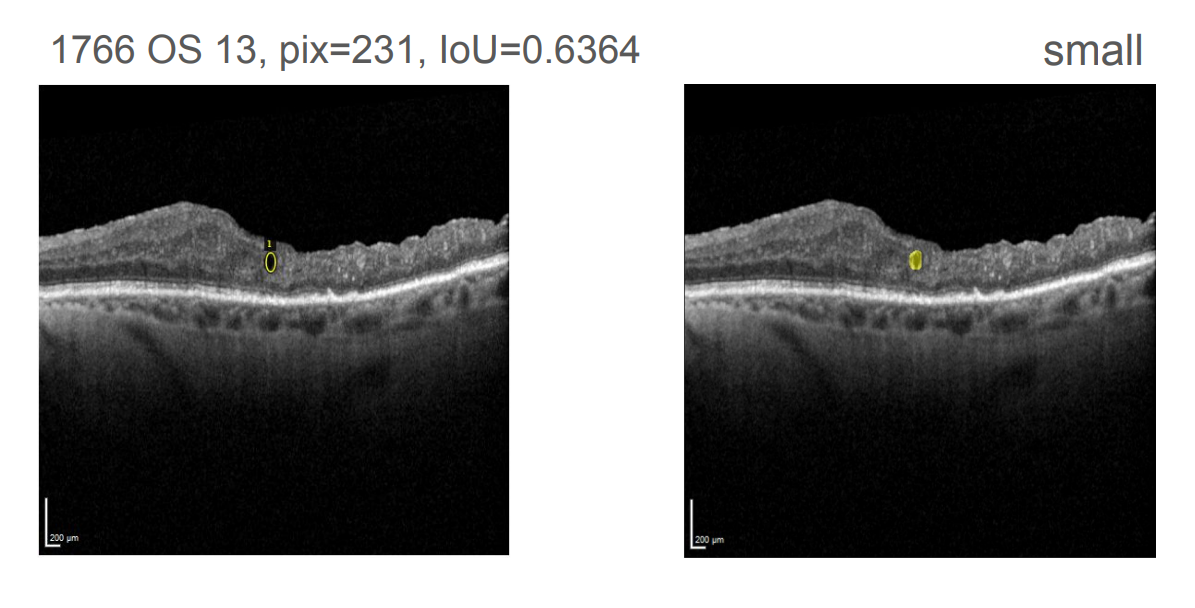
\includegraphics[width=0.75\textwidth]{./pic/Segmentierung/Segmentierungsergebnisse/21.PNG}
\caption{\label{fig:ergebnis_good1}Auszug eines Testbildes, mit einem kleinen Ödem. Links von Hand segmentiert, rechts Output des Segmentierungsmodells}
\end{figure}

In Abbildung \ref{fig:ergebnis_good2} ist ein mittelgroßes Ödem abgebildet, welches sich aus mehreren kleinen Ödemen zusammensetzt. Dies wurde als ein großes Ödem markiert, da die einzeln erkennbaren Flüssigkeitsansammlungen im Gesamtbild auch eine große Flüssigkeitskammer mit kleinen Trennwänden darstellen können. Ähnlich zu der Segmentierung wurde auch die Erkennung und Ausmessung durch das Modell vorgenommen. Bei ähnlichen Bildern zeigt sich, dass in manchen Fällen die schwarzen Flächen einzeln erkannt werden. Diese Unregelmäßigkeit lässt sich wahrscheinlich auf die unterschiedliche Segmentierungsart von Hand zurückführen und muss bei der Bewertung einer Verlaufskontrolle berücksichtigt werden. Da im Rahmen der Verlaufskontrolle stets alle 25 Bilder ins Gewicht fallen und solche Ödeme meist auf mehreren Bildern sichtbar sind, besteht die Möglichkeit, dass dieser Effekt durch die Aufsummierung im Endergebnis abgeschwächt wird.\newline
\begin{figure}[h]
\centering
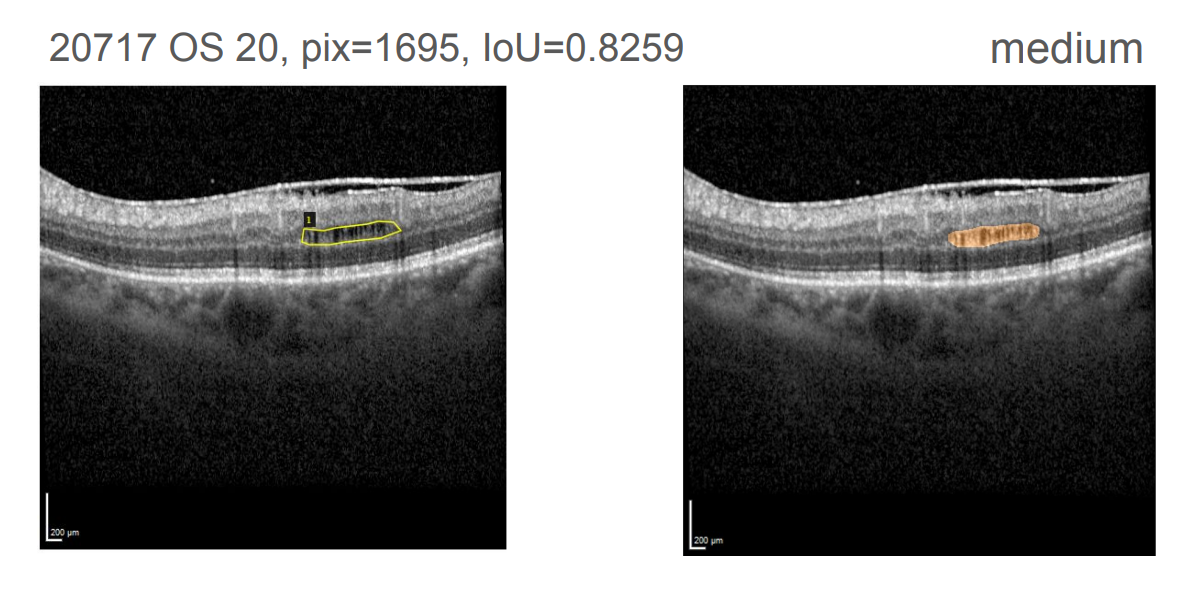
\includegraphics[width=0.75\textwidth]{./pic/Segmentierung/Segmentierungsergebnisse/38.PNG}
\caption{\label{fig:ergebnis_good2}Testbild, welches eine mittlere Größe aufweist. Links von Hand segmentiert, rechts Output des Segmentierungsmodells}
\end{figure}

Ein großes Ödem mit der besten IoU des Testdatensatzes ist in Abbildung \ref{fig:ergebnis_good3} zu sehen. Es zeigt sich eine gute Segmentierung der Fläche durch das Modell, welche so im Rahmen einer Verlaufskontrolle verwendbar wäre. Auch wenn die Ränder nicht immer perfekt getroffen wurden, zeigt sich durch die große absolute Größe des Ödems eine hohe IoU.\newline
\begin{figure}[ht!]
\centering
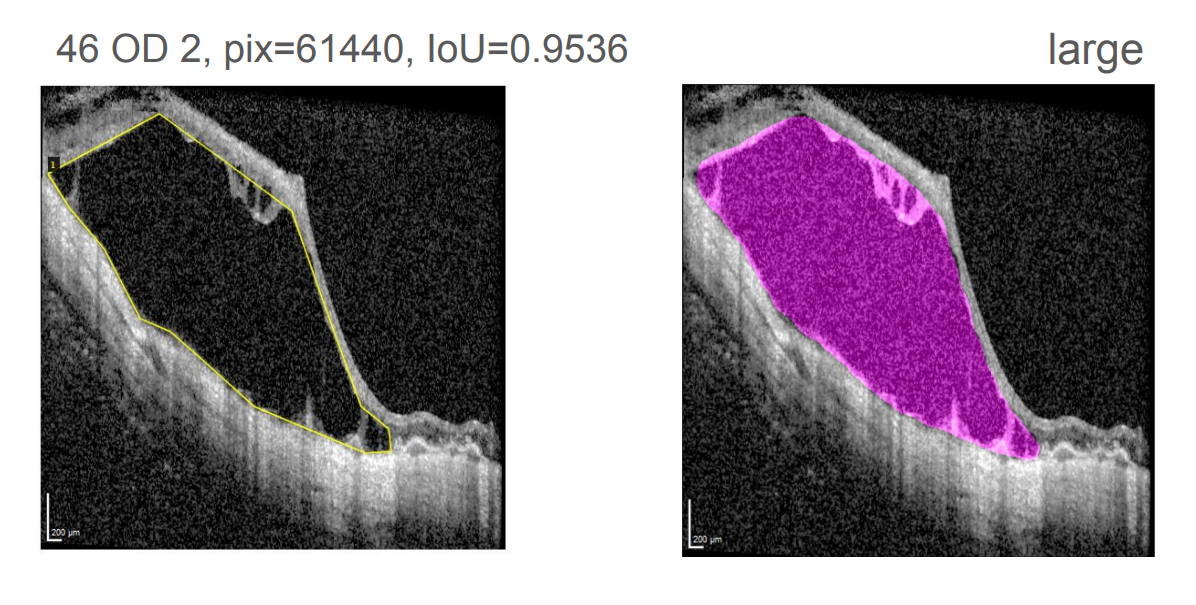
\includegraphics[width=0.75\textwidth]{./pic/Segmentierung/Segmentierungsergebnisse/50.PNG}
\caption{\label{fig:ergebnis_good3}Testbild, auf dem ein großes Segment erkennbar ist. Bei diesem Testbild wurde die höchste IoU erreicht. Links von Hand segmentiert, rechts Output des Segmentierungsmodells}
\end{figure}
Alle Segmentierungsergebnisse der 50 Testbilder befinden sich im Anhang.
%TODO Anhang



\newpage
%TODO remove newpage
\section{Grenzen der Segmentierung und Lösungsvorschläge}

% Häufige Fehler des Modells: ...

% Auf Augenebene hohe Sensitivität, jedoch geringe Spezifität
% Lösung: Einzelne falsch positive Ergebnisse geringer in das Endergebnis einfließen lassen (Spezifitiät verbessern)
Eine Schwäche des Modells ist derzeitig die geringe Spezifität. Wie bereits im Ergebnisteil beschrieben, werden von dem Modell aktuell noch viele der eigentlich negativen Bilder als falsch positive erkannt. 
Um dem entgegen zu wirken, wäre es denkbar einzelne falsch positive Ergebnisse geringer in das Endergebnis einfließen zu lassen. 


% Auswertung der Testdaten ist aufgrund geringer Datenmenge mit Unsicherheit behaftet
% -> Mehr Daten, mehr Training, mehr Test
Bei Deep-Learning-Methoden stellt eine geringe Menge an Testdaten häufig ein Problem dar. 
Da für das Training von dem Gesamtdatensatz nur etwa 5600 Bilder verwendet werden können, wäre es sinnvoll die Menge der Bilder um ein Vielfaches zu erhöhen. Durch das Trainieren des Netzes mit einem umfangreicherem Datensatz, werden robustere Ergebnisse erwartet, die auch die Problematik der geringen Spezifität abfangen sollte. 
Eine weitere Möglichkeit die Menge der Daten zu vervielfältigen ist es die vorhandenen Bilder zu augmentieren. 





\section{Zweites Training des Mask R-CNN}

% Aufgrund der geringen Testmenge: 2. Training mit mehr Testdaten
% 1000 Testbilder
% 4000 Trainingsbilder
% Architektur Modell des MRCNN wurde nich verändert
% -> für repräsentativere Ergebnisse
% leichte Verschlechterung der Ergebnisse
% Training beriets Optimiert -> kein overfitting siehe Grafik. 
% Modell verbessern durch augmentierte Daten

% Da dieses Ergebnis somit eine statistische Schätzung mit geringem Stichprobenumfang darstellt, ist dieses Ergebnis mit Unsicherheit behaftet.
Wie im Unterkapitel \ref{Segmentierung als binärer Klassifizierer} der Evaluierung bereits beschrieben, stellt bei dem trainierten Mask R-CNN Modell derzeit der geringe Stichprobenumfang noch ein Problem bei der Evaluierung dar. Die Ergebnisse sind bei einem zu geringen Testdatensatz noch mit Unsicherheit behaftet. 
Daher wurde das Modell erneut trainiert und dabei nun der Umfang an Testbildern erhöht.
Dabei wurden 1000 OCT-Bilder mit Ödemen dem Trainigsdatensatz entnommen, die später zur Evaluierung genutzt wurden. 
Somit hat sich der Umfang der Daten zum Trainieren des MRCNN-Modells auf 4598 Bilder verringert. Dies führt zwangsläufig zu einer Verschlechterung des Modells. Dafür sind die Ergebnisse dieses Modells aussagekräftiger und robuster. 

Das Vorgehen zum Trainieren des Modells wurde nicht verändert und es wurden die exakt gleichen Parameter verwendet, sodass eine Vergleichbarkeit sichergestellt ist. 
Im folgenden Abschnitt werden die Ergebnisse des zweiten Trainings vorgestellt und zum den Ergebnissen des ersten Modells verglichen. 

In Abbildung \ref{fig:iou_tp_t2} wird die Maßzahl IoU auf den Testdaten gezeigt. 
In dem neu trainierten Modell liegt der Median der IoU bei 0.68 und der Mittelwert bei 0.62.
Zum Vegleich: Im ersten Modell liegt der Median der IoU bei 0.70 und der Mittelwert bei 0.63 (siehe Abbildung \ref{fig:iou_testonly50}).
Somit hat sich das Modell auf Basis der Testdaten nur geringfügig verschlechtert. 




\begin{figure}[H]
\centering
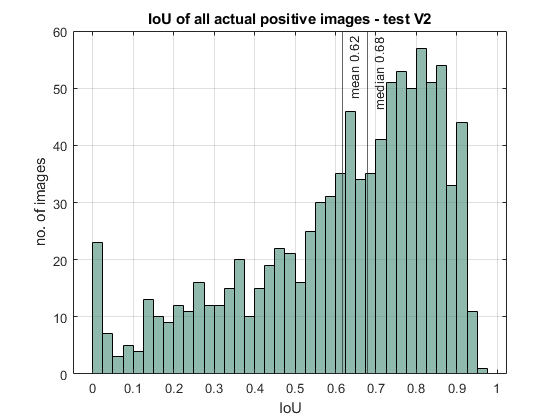
\includegraphics[width=0.7\textwidth]{./pic/Segmentierung/iou_all_tp_train2.png}
\caption{\label{fig:iou_tp_t2}Histogramm der Intersection over Union als Ergebnis der Evaluation aller positiven
Testdaten des zweiten Modells. Auf der Abszisse ist die Intersection over Union, auf der Ordinate die Anzahl der Bilder
aufgetragen. }
\end{figure}


In der nächsten Abbildung wurde wie auch in der Auswertung des ersten Modells die IoU je Ödemgröße ausgewertet. 
Wie auch zuvor schon ist hier zu sehen, dass die Genauigkeit der IoU steigt je größer das zu segmentierte Ödem ist. 
Insgesamt ist aber auch hier wieder eine Verschlechterung um etwa 10\% je Wert zu erkennen. Dabei sinkt die Ungenauigeit mit zunehmender Ödemgröße.



\begin{figure}[H]
\centering
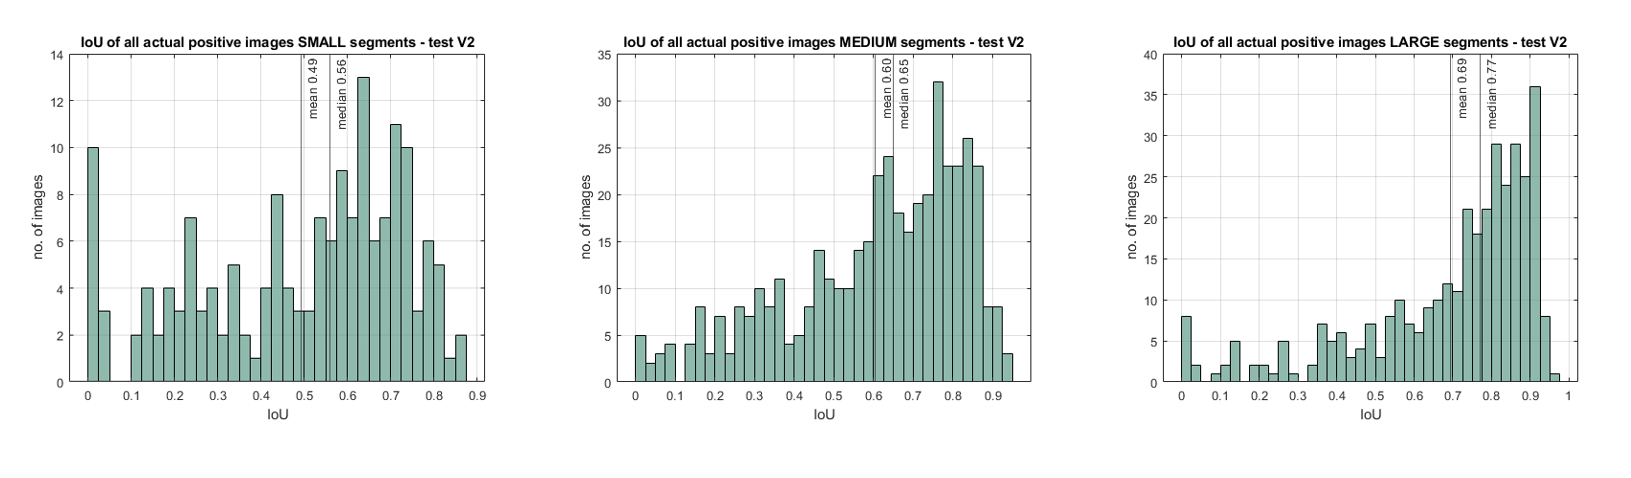
\includegraphics[width=\textwidth]{./pic/Segmentierung/iou_all_sizes_train2.png}
\caption{\label{fig:iou_allsizes_t2}  Histogramm der Intersection over Union (IoU) als Ergebnis der Evaluation aller original positiven Bilder des zweiten Modells. }
\end{figure}


Bei der Auswertung der Performance des neuen Modells auf den negativen Bildern, zeigt sich ein ähnliches Ergebnis. 
Das zweite Modell erreicht eine hohe Spezifität von 90\%. Das ist nur ein Prozentpunkt schlechter als die des ersten Modells. Somit ist die Performance des neu trainierten Modells doch vergleichbar mit dem Vorgängermodell. 
In Abbildung \ref{fig:iou_neg_t2} wird die Rate der richtig und falsch klassifizierten Bildern durch das neue MRCNN-Modell gezeigt. 
Dabei sind die falsch positiven Bilder nach der Größe der gefundenen Ödeme unterteilt. Hierbei ist erneut zu erkennen, dass die Unsicherheit bei kleinen Ödemen größer ist. Kleine (weniger und gleich 800 Pixel) und mittelgroße Ödeme machen einen Anteil von etwa jeweils 4\% unter den falsch positiven aus. Große Ödeme dagegen nur knapp 3\%.




\begin{figure}[H]
\centering
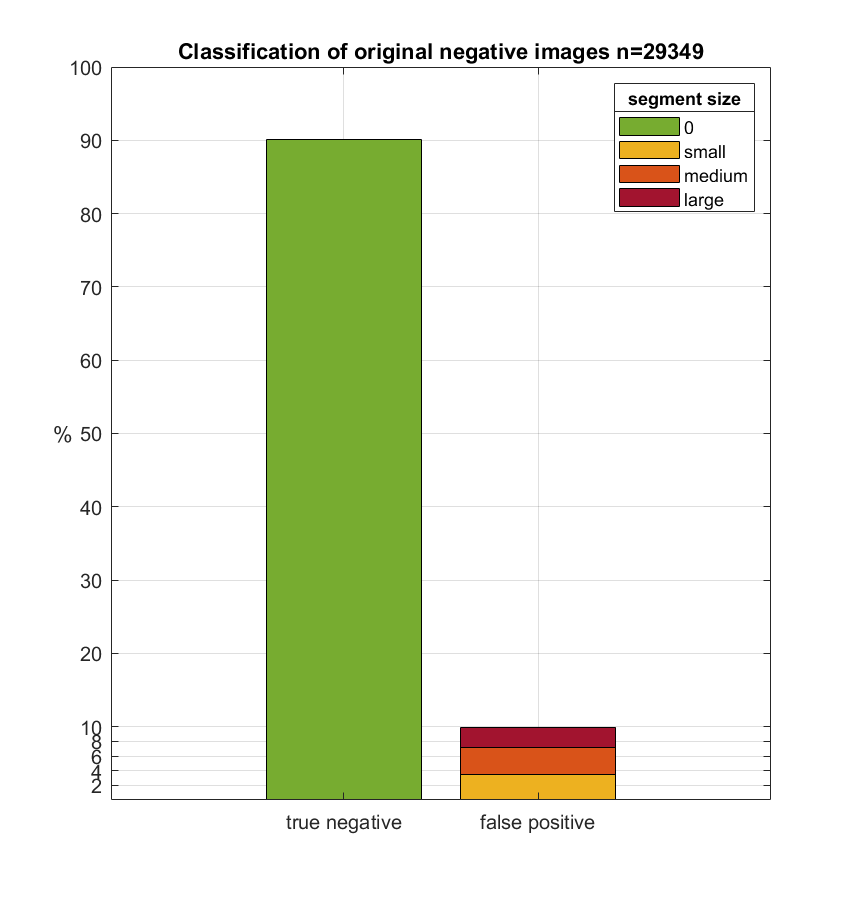
\includegraphics[width=0.6\textwidth]{./pic/Segmentierung/eval_neg_train2.png}
\caption{\label{fig:iou_neg_t2} Balkendiagramm der Anteile richtig und falsch klassifizierter negativen OCT-Bilder des neu trainierten Modells. Links die echt negativ und Rechts die falsch positiv Rate. Die falsch positiv Rate wird unterteilt dargestellt nach Größe der Segmente. }
\end{figure}



Somit hat sich eine Verschlechterung des Modells aufgrund der deutlichen Verkleinerung des Trainingsdatensatzes bestätigt, jedoch fällt diese in einem geringeren Maße aus als erwartet. 
Die mit diesem Modell ermittelten Ergebnisse sind als aussagekräftiger im Vergleich zum ersten Modell zu betrachten. Dennoch beweist die nur geringe Abweichung bereits eine gewisse Robustheit beider Modelle. 